%+------------+------------+--------------------------------------------------------------------+
%|    Data    |  Autoriai  |                            Pakeitimai                              |
%+------------+------------+--------------------------------------------------------------------+
%| 2016-09-15 | Visi       | Temos pasirinkimas, aprašo rašymas                                 |
%+------------+------------+--------------------------------------------------------------------+
%| 2016-09-22 | Visi       | Išorinė verslo proceso analizė                                     |
%+------------+------------+--------------------------------------------------------------------+
%| 2016-09-24 | Gabrielė   | Įeiga, išeiga, kritinės reikšmės, matavimų lentelė                 |
%+------------+------------+--------------------------------------------------------------------+
%| 2016-09-25 | Margiris   | Konkurentų sistemų veikimo analizė                                 |
%+------------+------------+--------------------------------------------------------------------+
%| 2016-09-27 | Vytautas   | Verslo proceso aprašo papildymas, minimalūs formatavimo pakeitimai |
%+------------+------------+--------------------------------------------------------------------+
%| 2016-09-28 | Gabrielė   | Papildyta apie Žiemos olimpines žaidynes. Anotacija, įvadas        |
%+------------+------------+--------------------------------------------------------------------+
%| 2016-09-29 | Vytautas   | UML klasių diagrama                                                |
%|            | Gabrielė   |                                                                    |
%+------------+------------+--------------------------------------------------------------------+
%| 2016-09-29 | Margiris   | Neišnaudotų galimybių, išorinio reguliavimo papildymas             |
%+------------+------------+--------------------------------------------------------------------+
%| 2016-09-29 | Vytautas   | Turinys                                                            |
%+------------+------------+--------------------------------------------------------------------+
%| 2016-09-29 | Gabijus    | Konkurentų sistemų veikimo analizė                                 |
%+------------+------------+--------------------------------------------------------------------+
%| 2016-09-29 | Vytautas   | Google docs variantas pakeistas į LaTeX                            |
%+------------+------------+--------------------------------------------------------------------+
%| 2016-10-01 | Gabijus    | Dalykinės srities žodynas                                          |
%+------------+------------+--------------------------------------------------------------------+
%|            | Vytautas   |                                                                    |
%| 2016-10-02 | Margiris   | Užduotys                                                           |
%|            | Gabrielė   |                                                                    |
%+------------+------------+--------------------------------------------------------------------+
%| 2016-10-02 | Vytautas   | UML užduočių diagrama                                              |
%+------------+------------+--------------------------------------------------------------------+
%|            | Vytautas   |                                                                    |
%| 2016-10-02 | Margiris   | Užduočių aprašymas                                                 |
%|            | Gabijus    |                                                                    |
%+------------+------------+--------------------------------------------------------------------+
%| 2016-10-02 | Visi       | Užduočių vykdymo scenarijaus UML diagrama                          |
%+------------+------------+--------------------------------------------------------------------+
%| 2016-10-04 | Visi       | Refuctoring                                                        |
%+------------+------------+--------------------------------------------------------------------+
%| 2016-MM-DD | VARDAI     | TEKSTAS                                                            |
%+------------+------------+--------------------------------------------------------------------+
%| 2016-MM-DD | VARDAI     | TEKSTAS                                                            |
%+------------+------------+--------------------------------------------------------------------+
%| 2016-MM-DD | VARDAI     | TEKSTAS                                                            |
%+------------+------------+--------------------------------------------------------------------+
%| 2016-MM-DD | VARDAI     | TEKSTAS                                                            |
%+------------+------------+--------------------------------------------------------------------+
%| 2016-MM-DD | VARDAI     | TEKSTAS                                                            |
%+------------+------------+--------------------------------------------------------------------+
%| 2016-MM-DD | VARDAI     | TEKSTAS                                                            |
%+------------+------------+--------------------------------------------------------------------+
%| 2016-MM-DD | VARDAI     | TEKSTAS                                                            |
%+------------+------------+--------------------------------------------------------------------+
%| 2016-MM-DD | VARDAI     | TEKSTAS                                                            |
%+------------+------------+--------------------------------------------------------------------+
%| 2016-MM-DD | VARDAI     | TEKSTAS                                                            |
%+------------+------------+--------------------------------------------------------------------+
%| 2016-MM-DD | VARDAI     | TEKSTAS                                                            |
%+------------+------------+--------------------------------------------------------------------+
%| 2016-MM-DD | VARDAI     | TEKSTAS                                                            |
%+------------+------------+--------------------------------------------------------------------+
%| 2016-MM-DD | VARDAI     | TEKSTAS                                                            |
%+------------+------------+--------------------------------------------------------------------+
%| 2016-MM-DD | VARDAI     | TEKSTAS                                                            |
%+------------+------------+--------------------------------------------------------------------+
%| 2016-MM-DD | VARDAI     | TEKSTAS                                                            |
%+------------+------------+--------------------------------------------------------------------+
%| 2016-MM-DD | VARDAI     | TEKSTAS                                                            |
%+------------+------------+--------------------------------------------------------------------+

\documentclass{VUMIFPSkursinis}
\usepackage{algorithmicx}
\usepackage{algorithm}
\usepackage{algpseudocode}
\usepackage{amsfonts}
\usepackage{amsmath}
\usepackage{booktabs}
\usepackage{blindtext}
\usepackage{bm}
\usepackage{caption}
\usepackage{color}
\usepackage{float}
\usepackage{graphicx}
\usepackage{listings}
\usepackage{multirow}
\usepackage{scrextend}
\usepackage{subfig}
\usepackage{wrapfig}
\usepackage{longtable}
\usepackage{tabularx}
\usepackage{enumitem}

% Titulinio aprašas
\university{Vilniaus universitetas}
\faculty{Matematikos ir informatikos fakultetas}
\department{Programų sistemų katedra}
\papertype{1 laboratorinis darbas}
\title{Lietuvos Nacionalinė Sporto Organizacija }
\titleineng{Lithuanian National Sports Organization}
\status{2 kurso 5 grupės studentai}
\author{Margiris Strakšys}
\secondauthor{Gabrielė Saletytė}
\thirdauthor{Vytautas Strimaitis}
\fourthauthor{Gabijus Arūnas Šukaitis}
\supervisor{jaun. mokslo darbuotojas Vytautas Valaitis}
\date{Vilnius – \the\year}

% Nustatymai
% \setmainfont{Palemonas}   % Pakeisti teksto šriftą į Palemonas (turi būti įdiegtas sistemoje)
%\bibliography{bibliografija}


%==========================================================================> Dokumento pradžia <========================================================================
\begin{document}
\maketitle

\tableofcontents

\sectionnonum{Anotacija} \label{anotacija}
  Šiuo darbu siekiama sukurti organizaciją, rengiančią olimpinio tipo varžybas Lietuvoje. Projekto tikslas - išanalizuoti esamų
  konkurentų darbus, jų pasiekimus ir sukurti naują modernų projektą, pritrauksiantį ne tik tradicinių, fizinių sporto šakų
  atstovus, tačiau ir E-sporto aistruolius.

\sectionnonum{Įvadas} \label{ivadas}
  \subsection*{Programų sistemos pavadinimas} \label{ivadas_pavadinimas}
    „Lietuvos nacionalinė sporto organizcija” (sutrumpintas sistemos pavadinimas - „LtNSO”).

  \subsection*{Darbo tikslas} \label{ivadas_tikslas}
    Išanalizuoti esamą įvairių varžybų situaciją ir pasitelkus analizę sukurti naują
    organizaciją, atnešančią Lietuvai naujas, inovatyvias idėjas, išpildyti įvaraus pobūdžio sportininkų lūkesčius.

  \subsection*{Temos aktualumas} \label{ivadas_aktualumas}
    Pasaulyje vyksta įvairaus tipo sporto renginių - nuo vienos iki kelių sporto šakų, nuo vietinių iki pasaulinio
    lygio. Tačiau visi Lietuvoje vykstantys sporto renginiai yra dažniausiai tik vienos sporto šakos ir nedidelio masto.
    Egzistuoja ryškus didelių, visą šalį apimančių žaidynių trūkumas. Taip pat, pasaulinio lygio renginiai teikia galimybę
    sekti sportininkų rezultatus ir stebėti pačias varžybas, o Lietuvoje tokios sistemos dar nėra gerai išvystytos.

  \subsection*{Siekiami rezultatai} \label{ivadas_siekiamiRezultatai}
    Lietuvos Nacionalinė Sporto Organizacija siekia pagerinti Lietuvos piliečių susidomėjimą įvairaus pobūdžio sportu,
    rengti visiems prieinamas sporto žaidynes bei sukurti jas apjungiančią programų sistemą. Tikimasi, kad sportininkai
    aktyviai dalyvaus varžybose ir sulauks didelio palaikymo bei paramos iš savivaldybių.

  \subsection*{Darbo pagrindas}  \label{ivadas_darboPagrindas} % [TODO] ar reikia?
    Dokumentas parengtas kaip programų sistemų inžinerijos laboratorinis darbas.

\section{Verslo proceso aprašas} \label{versloProcesoAprasas} % daugiau apie pačią problemą, kitką iškelt kažkur (pvz tikslus -> Verslo sistemos reguliavimo ir įvaizdžio valdymo tikslai ...)
  \subsection*{Nagrinėjamos srities apibrėžimas} \label{versloProcesoAprasas_sritiesApibrezimas}
    Sportas, sportiškai aktyvūs žmonės, sporto renginiai.
  \subsection*{Dalykinė sritis} \label{versloProcesoAprasas_dalykineSritis}
    Sportas Lietuvoje.
  \subsection*{Probleminė sritis} \label{versloProcesoAprasas_problemineSritis}
    Plataus spektro sportinių varžybų organizavimas.
  \subsection*{Aprašymas} \label{versloProcesoAprasas_aprasymas}
    Šiame verslo projekte nagrinėjamas sporto renginių organizavimas siekiant populiarinti sportą Lietuvoje,
    taip pat sportininkų reitingavimas ir lengvas renginių stebėjimas išoriniams žiūrovams. Šiuo metu Lietuvoje
    vykstantys sporto renginiai yra arba tik vienos sporto šakos, arba vos kelių, ir dažniausiai nėra visos
    šalies masto. Be to, norint dalyvauti tose keliose šalies lygio varžybose visų pirma reikia dalyvauti mažesnėse
    rungtynėse ir įveikti atranką. Tačiau mažosiose varžybose dalyvauti daugelis žmonių nenori, taip pat nėra bendros
    sistemos, apjungiančios visų tipų varžybas, leidžiančios kiekvienam norinčiam užsiregistruoti ir išbandyti savo jėgas,
    sekti rezultatus, stebėti pačias rungtynes.

    Pasaulyje yra panašaus tipo renginių, apimančių ne vieną sporto šaką ir teikiančių galimybę stebėti varžybas visiems
    norintiems. Jose rungiasi geriausi atletai iš daugelio valstybių, rungtynes stebėti bei sekti rezultatus gali žiūrovai
    iš viso pasaulio. Tačiau toks didelis renginio mastas kelia ir problemų - jose fiziškai negali dalyvauti bet kuris
    norintis žmogus, nes tiesiog nėra tiek daug vietos. Iki šių varžybų reikia įveikti savo šalies etapą ir tik tada yra
    suteikiama teisė dalyvauti.

\section{Išorinė verslo proceso analizė} \label{isorineVersloProcesoAnalize}
  \subsection{Verslo sistemos įeigos, išeigos, reguliavimo ir įvaizdžio valdymo tikslai} \label{isorineVersloProcesoAnalize_ieigosIseigosValdymoTikslai}
    \subsubsection*{Įeiga} \label{isorineVersloProcesoAnalize_ieigosIseigosValdymoTikslai_ieiga}
      \begin{enumerate}
        \item Rėmėjai
        \item Žiūrovai
        \item Kitos sporto organizacijos
        \item Dalyviai
      \end{enumerate}
    \subsubsection*{Išeiga} \label{isorineVersloProcesoAnalize_ieigosIseigosValdymoTikslai_iseig}
      \begin{enumerate}
        \item Suorganizuotos varžybos
        \item Prizai
        \item Žmonių atsiliepimai
        \item Motyvacija dalyviams
      \end{enumerate}
    \subsubsection*{Sistemos reguliavimas} \label{isorineVersloProcesoAnalize_ieigosIseigosValdymoTikslai_reguliavimas}
      \begin{enumerate}
        \item Finansavimas
        \item Nekilnojamojo turto nuoma
      \end{enumerate}
    \subsubsection*{Sistemos įvaizdžio valdymo tikslai} \label{isorineVersloProcesoAnalize_ieigosIseigosValdymoTikslai_ivaizdzioValdymoTikslai}
      \begin{enumerate}
        \item Atsiliepimai žiniasklaidoje
        \item Reklamavimasis socialiniuose tinkluose
        \item Rėmėjų steigiami prizai
        \item Lietuvos sporto istorija
      \end{enumerate}
  \subsection{Esamų sistemų analizė} \label{isorineVersloProcesoAnalize_esamuSistemuAnalize}
    Šiuo metu Lietuvoje bei visame pasaulyje egzistuoja įvairaus tipo varžybų organizacijos, pavyzdžiui, krepšinio, futbolo, plaukimo čempionatai ir t.t.
    Tačiau pagrindinės sistemos, kurios bus analizuojamos yra tradicinės olimpinės žaidynės bei jungtiniai E-sporto turnyrai.
    \subsubsection*{Olimpinės žaidynės} \label{isorineVersloProcesoAnalize_esamuSistemuAnalize_olimpines}
      \subsubsubsection*{Sistemos veikimas} \label{isorineVersloProcesoAnalize_esamuSistemuAnalize_olimpines_veikimas}
        Vasaros olimpinės žaidynės yra tarptautinės varžybos, rengiamos kas ketverius metus nuo 1904 m.  Šios žaidynės yra laiko patikrintos ir populiarios
        visame pasaulyje. Laukiant žaidynių vyksta kvalifikaciniai turnyrai bei normatyvų vykdymai,  skirti išsiaiškinti, kurie atletai yra verti dalyvauti ir
        vyks į olimpines žaidynes su savo šalies nacionaline komanda. Žaidynės prasideda iškilminga atidarymo ceremonija, kurios metu vyksta šalių delegacijų
        eitynės  kurių pabaigoje įžiebiama olimpinė ugnis. Visos varžybos vyksta apie tris savaites ir pasibaigia šventiška uždarymo ceremonija.
      \subsubsubsection*{Sistemos trūkumai ir kylančios problemos} \label{isorineVersloProcesoAnalize_esamuSistemuAnalize_olimpines_trukumai}
        Olimpinių žaidynių metu vyksta įvairaus tipo varžybos, tačiau daugybė sporto šakų yra užmirštos. Nors šios žaidynės vyksta ilgą laiką ir yra
        populiarios visame pasaulyje, tačiau jos tampa vis mažiau pritaikytos šiuolaikiniam žmogui, kadangi vyksta vis tos pačios nusistovėjusios varžybos ir
        neatsiranda naujų, modernių rungčių. Šiuolaikiniame pasaulyje technologijos sparčiai tobulėja, todėl beveik kiekvieną dieną atsiranda naujų sporto šakų,
        kurios neturi galimybės patekti į Olimpinių žaidynių sudėtį.

        Kadangi Olimpinės žaidynės yra prestižinis renginys, juo domisi žmonės iš viso pasaulio. Norinčių dalyvauti Lietuvos bei kitų valstybių piliečių yra
        tūkstančiai, bet tik maža dalis jų gauna tokią galimybę. Taip yra todėl, kad šios žaidynės yra pasaulinis renginys, o panašaus tipo smulkesni renginiai
        nėra vykdomi. 

        Daugelis žaidynių mėgėjų, norinčių patekti į varžybas, turi mokėti nemažas sumas tam, kad galėtų gyvai pasižiūrėti mėgiamas rungtynes. Negalintys sau
        leisti šios pramogos, žiūrovai renkasi stebėti varžybas namuose. Visa tai yra nekomfortabilu, kadangi ekranas neatstoja dalyvavimo renginyje gyvai.
        Negana to, daugelis rungčių vyksta nepatogiu laiku (naktį ar darbo metu), todėl daugelis neturi galimybės pasižiūrėti žaidynių tiesiogiai.
    \subsubsection*{E-sportas: "Blizzcon"} \label{isorineVersloProcesoAnalize_esamuSistemuAnalize_blizzcon}
      \subsubsubsection*{Sistemos veikimas} \label{isorineVersloProcesoAnalize_esamuSistemuAnalize_blizzcon_veikimas}
        ,,Blizzcon'' - „Blizzard” kopanijos organizuojamas renginys, kurio metu vyksta visų „Blizzard” organizacijos sukurtų kompiuterinių žaidimų varžybos.
        Jos vyksta nuo 2006 m. Bilietai į šį renginį yra išparduodami per kelias dienas ir po to perpardavinėjami internete už didesnę kainą. Tai rodo,
        kad įvykis yra itin populiarus, net ir neturėdamas gilių šaknų. Pats renginys vyksta vieną savaitgalį, varžybos transliuojamos internetu ir turi
        daug kanalų, kad būtų galima žiūrėti tiek kokias nori varžybas, tiek kokia nori kalba (6 populiariausios kalbos pasaulyje).
      \subsubsubsection*{Sistemos trūkumai ir kylančios problemos} \label{isorineVersloProcesoAnalize_esamuSistemuAnalize_blizzcon_trukumai}
        ,,Blizzcon'' yra gana naujas renginys, todėl jis susiduria su daug problemų. Jiems reikia ieškoti rėmėjų, nes dar nėra susiformavusi tradicija
        paremti šį renginį. Rėmėjų sritis nėra didelė, nes tai elektroninio sporto renginys ir dažniausiai finansavimą skiria su informacinėmis technologijomis
        susijusios įmonės. Kita problema yra visų žaidimų stebėjimo populiarinimas - kai kurie susilaukia didelio dėmėsio, o kiti lieka nuošalyje. Kadangi tai
        kompanijos renginys, ji norėtų, kad visi jos išleisti žaidimai turėtų paklausą.
    \subsubsection*{"Starladder"} \label{isorineVersloProcesoAnalize_esamuSistemuAnalize_starladder}
      \subsubsubsection*{Sistemos veikimas} \label{isorineVersloProcesoAnalize_esamuSistemuAnalize_starladder_veikimas}
       ,,Starladder'' vyksta kitaip nei ,,Blizzcon''. Daugiausia varžybų vyksta internetu, kai komandos neatvažiuoja  į renginį, o žaidžia savo šalyse.
        Varžybos matomos internetu per įvairius kanalus. Šis renginys apima tris bene didžiausias E-sporto platformas: ,,CS:GO'', ,,Dota2'' ir ,,Hearthstone''.
        Vieną kartą per metus įvyksta ir kiekvieno iš šių žaidimų turnyras, kuriame komandos ir individualūs žaidėjai turi atvažiuoti į patį renginį. Jis
        vyksta vieną savaitgalį dažniausiai arenoje, į kurią žiūrovai gali nusipirkti bilietą.
      \subsubsubsection*{Sistemos trūkumai ir kylančios problemos} \label{isorineVersloProcesoAnalize_esamuSistemuAnalize_starladder_trukumai}
        ,,Starladder'' yra beveik visus metus vykstantis renginys, todėl sunku pritraukti didelį kiekį žiūrovų į kiekvieną iš mažųjų renginių. Pagrindinio
        renginio lokacija, kuri yra Kijevas (Ukraina), yra problematiška, nes pati šalis nėra stabili ir sportininkams bei žiūrovams iš kitų šalių, gali būti
        nekomfortabilu vykti į tokią šalį.
  \subsection{Metrikos} \label{isorineVersloProcesoAnalize_metrikos}
    %\renewcommand{\tabularxcolumn}[1]{m{#1}}
    %\begin{tabularx} {.9\textwidth}{ | >{\bfseries\hsize=.1\hsize}c
    %                                 | >{\hsize=.4\hsize}c
    %                                 | >{\hsize=.4\hsize}c
    %                                 | X | }
    %  \hline
    %  \textbf{Nr.} & \multicolumn{3}{|c|}{\textbf{Kokybė}} \\
    %  \hline
    %  \textbf{1}   & \multicolumn{3}{|c|}{\textbf{Patenkintų žiūrovų skaičius}} \\
    %  \hline
    %  {}           & \textbf{Matavimo vienetai}                     & $\frac{P}{N} \cdot 100\%$  & Žiūrovų, patenkintų žaidynėmis, dalis procentais \newline ABCD \newline Anotha one \\
    %  \cline{2-4}                    
    %  {}           & \textbf{Kritinės reikšmės}                     & \textbf{Geriausiu atveju}  & 10\% \\
    %  \cline{3-4}                    
    %  {}           & {}                                             & \textbf{Blogiausiu atveju} & 5\% \\
    %  \cline{2-4}
    %  {}           & \multicolumn{2}{|l|}{\textbf{Esamos reikšmės}} & 0\% \\
    %  \hline
    %\end{tabularx}
    %\renewcommand{\tabularxcolumn}[1]{p{#1}}
    
    \renewcommand{\tabularxcolumn}[1]{m{#1}}
    \begin{table}[H]
      \caption{Įeigų metrikos}
      \label{table:ieiga}
      \begin{tabularx} {.9\textwidth}{ | >{\bfseries\hsize=.1\hsize}c
                                      | >{\hsize=.4\hsize}c
                                      | >{\hsize=.4\hsize}c
                                      | X | }
        \hline
        \textbf{Nr.} & \multicolumn{3}{|c|}{\textbf{Įeiga}} \\
        \hline
        \textbf{1}   & \multicolumn{3}{|c|}{\textbf{Rėmėjai}} \\
        \hline
        {}           & \multicolumn{2}{|l|}{\textbf{Matavimo vienetai}} & Rėmėjų skaičius renginiui \\
        \cline{2-4}                    
        {}           & \textbf{Kritinės reikšmės}                       & \textbf{Geriausiu atveju}  & 15 rėmėjų \\
        \cline{3-4}                    
        {}           & {}                                               & \textbf{Blogiausiu atveju} & 0 rėmėjų \\
        \cline{2-4}
        {}           & \multicolumn{2}{|l|}{\textbf{Esamos reikšmės}}   & 7 rėmėjai \\
        \hline

        \textbf{2}   & \multicolumn{3}{|c|}{\textbf{Žiūrovai}} \\
        \hline
        {}           & \multicolumn{2}{|l|}{\textbf{Matavimo vienetai}} & Žiūrovų, stebinčių renginį, skaičius \\
        \cline{2-4}                    
        {}           & \textbf{Kritinės reikšmės}                       & \textbf{Geriausiu atveju}  & 50 mln. žiūrovų \\
        \cline{3-4}                    
        {}           & {}                                               & \textbf{Blogiausiu atveju} & 10 žiūrovų \\
        \cline{2-4}
        {}           & \multicolumn{2}{|l|}{\textbf{Esamos reikšmės}}   & 15 tūkst. žiūrovų \\
        \hline
        
        \textbf{3}   & \multicolumn{3}{|c|}{\textbf{Kitos sporto organizacijos}} \\
        \hline
        {}           & \multicolumn{2}{|l|}{\textbf{Matavimo vienetai}} & Sporto organizacijų, prisidedančių prie renginio, skaičius \\
        \cline{2-4}                      
        {}           & \textbf{Kritinės reikšmės}                       & \textbf{Geriausiu atveju}  & 42 sporto organizacijos \\
        \cline{3-4}                      
        {}           & {}                                               & \textbf{Blogiausiu atveju} & 0 sporto organizacijų \\
        \cline{2-4}  
        {}           & \multicolumn{2}{|l|}{\textbf{Esamos reikšmės}}   & 1 sporto organizacija \\
        \hline
        
        \textbf{4}   & \multicolumn{3}{|c|}{\textbf{Dalyviai}} \\
        \hline
        {}           & \multicolumn{2}{|l|}{\textbf{Matavimo vienetai}} & Žmonių, dalyvaujančių renginyje, skaičius \\
        \cline{2-4}                      
        {}           & \textbf{Kritinės reikšmės}                       & \textbf{Geriausiu atveju}  & 11,5 tūkst. dalyvių \\
        \cline{3-4}                      
        {}           & {}                                               & \textbf{Blogiausiu atveju} & 16 dalyvių \\
        \cline{2-4}  
        {}           & \multicolumn{2}{|l|}{\textbf{Esamos reikšmės}}   & 150 dalyvių \\
        \hline
      \end{tabularx}
    \end{table}
    

    
    \begin{table}[H]
      \caption{Išeigų metrikos}
      \label{table:iseiga}
      \begin{tabularx} {.9\textwidth}{ | >{\bfseries\hsize=.1\hsize}c
                                      | >{\hsize=.4\hsize}c
                                      | >{\hsize=.4\hsize}c
                                      | X | }
        \hline
        \textbf{Nr.} & \multicolumn{3}{|c|}{\textbf{Išeiga}} \\
        \hline
        \textbf{1}   & \multicolumn{3}{|c|}{\textbf{Suorganizuotos varžybos}} \\
        \hline
        {}           & \multicolumn{2}{|l|}{\textbf{Matavimo vienetai}} & Suorganizuotų varžybų skaičius \\
        \cline{2-4}                    
        {}           & \textbf{Kritinės reikšmės}                       & \textbf{Geriausiu atveju}  & 42 varžybos \\
        \cline{3-4}                    
        {}           & {}                                               & \textbf{Blogiausiu atveju} & 1 varžybos \\
        \cline{2-4}
        {}           & \multicolumn{2}{|l|}{\textbf{Esamos reikšmės}}   & 1 varžybos \\
        \hline

        \textbf{2}   & \multicolumn{3}{|c|}{\textbf{Prizai}} \\
        \hline
        {}           & \multicolumn{2}{|l|}{\textbf{Matavimo vienetai}} & Pinigų, skirtų apdovanojimams, kiekis eurais. \\
        \cline{2-4}                      
        {}           & \textbf{Kritinės reikšmės}                       & \textbf{Geriausiu atveju}  & 18 mln. € \\
        \cline{3-4}                      
        {}           & {}                                               & \textbf{Blogiausiu atveju} & 20 € \\
        \cline{2-4}  
        {}           & \multicolumn{2}{|l|}{\textbf{Esamos reikšmės}}   & 5 tūkst. € \\
        \hline
        
        \textbf{3}   & \multicolumn{3}{|c|}{\textbf{Teigiami žmonių atsiliepimai}} \\
        \hline
        {}           & \textbf{Matavimo vienetai}                       & $\frac{a}{n} \cdot 100\%$ & Teigiamų žmonių atsiliepimų dalis procentais. \newline $a$ - teigiamų atsiliepimų skaičius, \newline $n$ - bendras atsiliepimų skaičius. \\
        \cline{2-4}                      
        {}           & \textbf{Kritinės reikšmės}                       & \textbf{Geriausiu atveju}  & 100\% \\
        \cline{3-4}                      
        {}           & {}                                               & \textbf{Blogiausiu atveju} & 0\% \\
        \cline{2-4}  
        {}           & \multicolumn{2}{|l|}{\textbf{Esamos reikšmės}}   & 70\% \\
        \hline
        
        \textbf{4}   & \multicolumn{3}{|c|}{\textbf{Neigiami žmonių atsiliepimai}} \\
        \hline
        {}           & \textbf{Matavimo vienetai}                       & $\frac{a}{n} \cdot 100\%$ & Neigiamų žmonių atsiliepimų dalis procentais. \newline $a$ - neigiamų atsiliepimų skaičius, \newline $n$ - bendras atsiliepimų skaičius. \\
        \cline{2-4}                      
        {}           & \textbf{Kritinės reikšmės}                       & \textbf{Geriausiu atveju}  & 0\% \\
        \cline{3-4}                      
        {}           & {}                                               & \textbf{Blogiausiu atveju} & 100\% \\
        \cline{2-4}  
        {}           & \multicolumn{2}{|l|}{\textbf{Esamos reikšmės}}   & 30\% \\
        \hline
        
        \textbf{5}   & \multicolumn{3}{|c|}{\textbf{Motyvacija dalyviams}} \\
        \hline
        {}           & \textbf{Matavimo vienetai}                       & $(\frac{n_{d}}{n_{p}} - 1) \cdot 100\%$ & Dalyvių prieaugis per metus. \newline $n_{p}$ - dalyvių skaičius praeitais metais, \newline $n_{d}$ - dalyvių skaičius dabar. \\
        \cline{2-4}                      
        {}           & \textbf{Kritinės reikšmės}                       & \textbf{Geriausiu atveju}  & 15\% \\
        \cline{3-4}                      
        {}           & {}                                               & \textbf{Blogiausiu atveju} & -30\% \\
        \cline{2-4}  
        {}           & \multicolumn{2}{|l|}{\textbf{Esamos reikšmės}}   & 2\% \\
        \hline
      \end{tabularx}
    \end{table}
    
    
    
    \begin{table}[H]
      \caption{Sistemos reguliavimo metrikos}
      \label{table:reguliavimas}
      \begin{tabularx} {.9\textwidth}{ | >{\bfseries\hsize=.1\hsize}c
                                      | >{\hsize=.4\hsize}c
                                      | >{\hsize=.4\hsize}c
                                      | X | }
        \hline
        \textbf{Nr.} & \multicolumn{3}{|c|}{\textbf{Sistemos reguliavimas}} \\
        \hline
        \textbf{1}   & \multicolumn{3}{|c|}{\textbf{Finansavimas}} \\
        \hline
        {}           & \multicolumn{2}{|l|}{\textbf{Matavimo vienetai}} & Pinigų kiekis, gaunamas iš išorinių šaltinių vienam sezonui, eurais. \\
        \cline{2-4}                      
        {}           & \textbf{Kritinės reikšmės}                       & \textbf{Geriausiu atveju}  & 90 mln. € \\
        \cline{3-4}                      
        {}           & {}                                               & \textbf{Blogiausiu atveju} & 1 tūkst. € \\
        \cline{2-4}  
        {}           & \multicolumn{2}{|l|}{\textbf{Esamos reikšmės}}   & 1 mln. € \\
        \hline

        \textbf{2}   & \multicolumn{3}{|c|}{\textbf{Nekilnojamo turto nuoma}} \\
        \hline
        {}           & \multicolumn{2}{|l|}{\textbf{Matavimo vienetai}} & Pinigų kiekis, išleistas varžyboms reikalingo nekilnojamojo turto nuomai renginiui, eurais. \\
        \cline{2-4}                      
        {}           & \textbf{Kritinės reikšmės}                       & \textbf{Geriausiu atveju}  & 500 € \\
        \cline{3-4}                      
        {}           & {}                                               & \textbf{Blogiausiu atveju} & 10 mln. € \\
        \cline{2-4}  
        {}           & \multicolumn{2}{|l|}{\textbf{Esamos reikšmės}}   & 5 tūkst. € \\
        \hline
      \end{tabularx}
    \end{table}
    \renewcommand{\tabularxcolumn}[1]{p{#1}}

\section{Vidinė verslo proceso analizė} \label{vidineVersloProcesoAnalize}

  \subsection{Dalykinės srities statinė struktūra} \label{vidineVersloProcesoAnalize_statineStruktura}

    \subsubsection*{Dalykinės srities esybių žodynas} \label{vidineVersloProcesoAnalize_statineStruktura_zodynas}
      \begin{description}
			  \item[Žiūrovas] Žmogus, kuris stebi varžybas.
			  \item[Sirgalius] Žmogus, kuris palaiko atletus ar komandas ir stebi varžybas.
			  \item[Dalyvis] Žmogus, kuris dalyvauja varžybose.
			  \item[Prizininkas] Sportinio renginio dalyvis, gavęs apdovanojimą.
			  \item[Darbuotojas] Žmogus, kuris dirba renginyje.
			  \item[Nugalėtojas] Dalyvis, kuriam pavyko įveikti visus savo varžovus ir iškovoti pirmąją vietą.
			  \item[Tarptautinis sporto renginys] Sportinis renginys, kuriame dalyvauja sportininkai iš viso pasaulio.
			  \item[Regioninis sporto renginys] Sportinis renginys, vykstantis vieno regiono mastu.
			  \item[Nacionalinis sporto renginys] Sportinis renginys, vykstantis šalies mastu.
			  \item[Sporto renginys] Renginys, kurio metu vyksta sporto varžybos, į jį susirenka ir dalyviai , ir žiūrovai.
			  \item[Varžybos] Kokios nors sporto šakos renginys, kurio metu išsiaiškinamas nugalėtojas bei kiti prizininkai.
			  \item[Teisėjas] Darbuotojas, kuris prižiūri varžybų veiklą, užtikrina, kad dalyviai laikytųsi rungties taisyklių.
			  \item[Pagalbinis darbuotojas] Žmogus, kuris padeda teisėjui ir kitiems darbuotojams palaikyti tvarką per žaidynes.
			  \item[Sporto šaka] Sportinė veiklos sritis, kuri turi savo taisykles ir inventorių.
			  \item[Komandinio sporto šaka] Sporto šaka, kurioje varžosi dvi komandos.
			  \item[Indivualaus sporto šaka] Sporto šaka, kurioje sportininkai varžosi dviese vienas prieš kitą.
			  \item[Rėmėjas] Žmogus ar kompanija, kuris skiria pinigus žaidynėms, siekdamas reklamuotis arba tiesiog prisidėti prie sportiškesnės visuomenės.
			  \item[Organizatorius] Įstaiga, kuri rengia varžybas, duoda nurodymus darbuotojams, skiria prizus, moka algas ir yra pagrindinė institucija atsakinga už varžybų rengimą.
			  \item[Prizas] Dovana, kurią gauna varžybų nugalėtojas, ji gali buti piniginė, daiktinė.  
			\end{description}

    \subsubsection*{Dalykinės srities struktūra} \label{vidineVersloProcesoAnalize_statineStruktura_dalykinesSritiesStruktura}
    \begin{figure}[H]
      \centering
      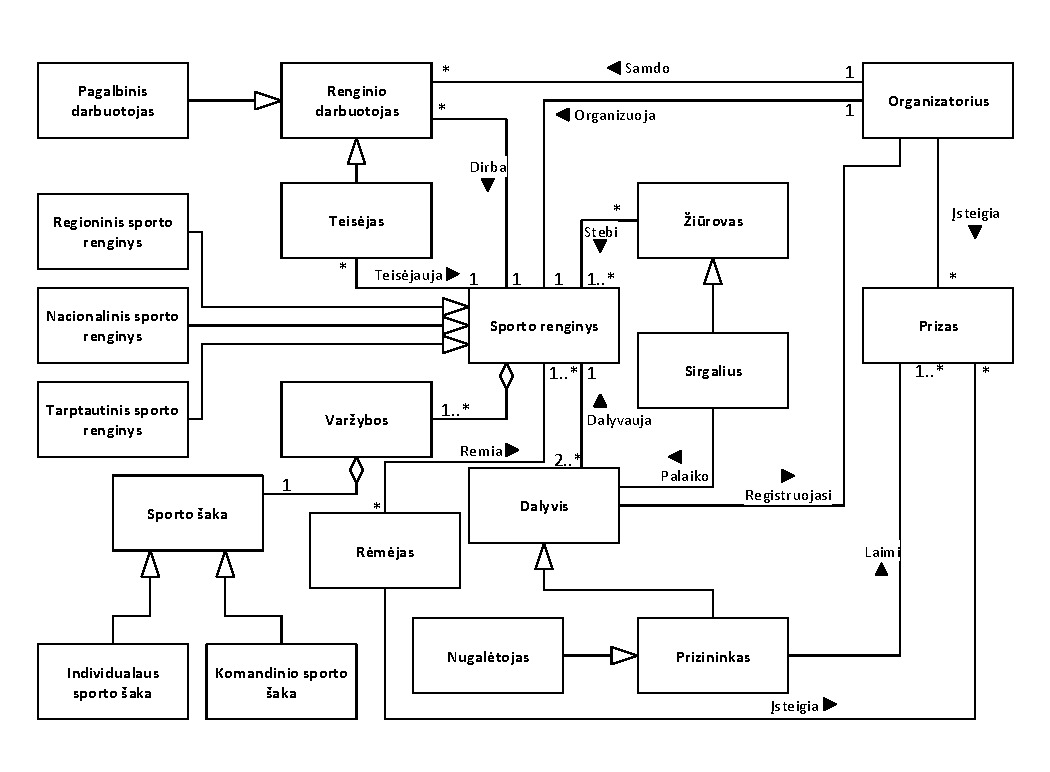
\includegraphics[width=\textwidth]{img/KlasiuDiagrama}
      \caption{UML klasių diagrama}
      \label{fig:klasiuDiagrama}
    \end{figure}
  \subsection{Užduotys} \label{vidineVersloProcesoAnalize_uzduotys}
    \subsubsection*{Pagrindinės sistemos užduotys ir su jomis susiję agentai} \label{vidineVersloProcesoAnalize_uzduotys_uzduotysIrAgentai}
      \renewcommand{\labelitemi}{$\bullet$}
      \renewcommand{\labelitemii}{$\circ$}
      \begin{itemize}
        \item Agentai:
          \begin{description}
            \item [$\circ$ Žiūrovas] Žmogus, priklausantis klasei \underline{žiūrovas}.
            \item [$\circ$ Dalyvis] Žmogus, priklausantis klasei \underline{dalyvis}.
            \item [$\circ$ Teisėjas] Žmogus, prižiūrintis varžybas. Priklauso klasei \underline{teisėjas}.
            \item [$\circ$ Rėmėjas] Žmogus ar organizacija, kuri teikia resursus siekdama palengvinti \underline{sporto renginio} organizavimą. Priklauso klasei \underline{rėmėjas}.
            \item [$\circ$ Organizatorius] Įmonė, atsakinga už \underline{sporto renginio} organizavimą. Priklauso klasei \underline{organizatorius}.
          \end{description}
        \item Užduotys:
          \begin{description}
            \item [$\circ$ Registruotis] \underline{Dalyvis} pateikia savo asmeninę informaciją \underline{organizatoriui}.
            \item [$\circ$ Gauti registracijos rezultatą] \underline{Dalyvis} gauna atsakymą iš \underline{organizatoriaus} apie jo registracijos būklę.
            \item [$\circ$ Dalyvauti] \underline{Dalyvis} atvyksta į \underline{varžybas} ir rungiasi su kitais \underline{dalyviais}.
            \item [$\circ$ Kovoti dėl aukščiausių vietų] \underline{Dalyvis} dalyvaudamas \underline{varžybose} siekia užimti kuo geresnę vietą ir iškovoti \underline{prizų}.
            \item [$\circ$ Teisėjauti] \underline{Teisėjas} prižiūri bendrą tvarką bei taisyklių laikymąsi \underline{varžybose}.
            \item [$\circ$ Fiksuoti rezultatus] \underline{Teisėjas} stebi \underline{varžybų} eigą ir fiksuoja \underline{dalyvių} rezultatus.
            \item [$\circ$ Stebėti] \underline{Žiūrovas} netiesiogiai dalyvauja \underline{sporto renginyje} jį stebėdamas gyvai ar per \underline{organizatorių} teikiamas medijos priemones.
            \item [$\circ$ Sekti rezultatus] \underline{Žiūrovas} stebi \underline{dalyvių} pasirodymus \underline{varžybose} ir seka jų rezultatus.
            \item [$\circ$ Steigti prizus] \underline{Rėmėjas} ar \underline{organizatorius} skiria pinigines ar daiktines dovanas, vėliau įteikiamas geriausiai pasirodžiusiems \underline{dalyviams}.
            \item [$\circ$ Nuomoti nekilnojamąjį turtą] \underline{Organizatorius} išnuomoja \underline{sporto renginiui} reikalingas dideles patalpas ir stadionus, kuriuose vyks \underline{varžybos}.
            \item [$\circ$ Remti renginį] \underline{Rėmėjai} suteikia finansinę paramą \underline{sporto renginio} \underline{organizatoriams} taip padėdami padengti \underline{renginio} išlaidas.
            \item [$\circ$ Ieškoti rėmėjų] \underline{Organizatoriai} ieško rėmėjų, kurie galėtų suteikti paramą \underline{sporto renginio} išlaidoms padengti.
            \item [$\circ$ Sudaryti renginio tvarkaraštį] \underline{Organizatoriai} iš anksto sudaro \underline{sporto renginio} tvarkaraštį, kuriame nurodomos konkrečių varžybų datos.
            \item [$\circ$ Apdovanoti nugalėtojus] \underline{Organizatoriai} ir \underline{rėmėjai} įteikia \underline{prizus} geriausiai kiekvienos \underline{sporto šakos} \underline{varžybose} pasirodžiusiems \underline{dalyviams}.
          \end{description}
      \end{itemize}

    \subsubsection*{Pagrindinės užduotys} \label{vidineVersloProcesoAnalize_uzduotys_pagrindinesUzduotys}
      \subsubsubsection*{Renginio organizavimas}
        \begin{figure}[H]
          \centering
          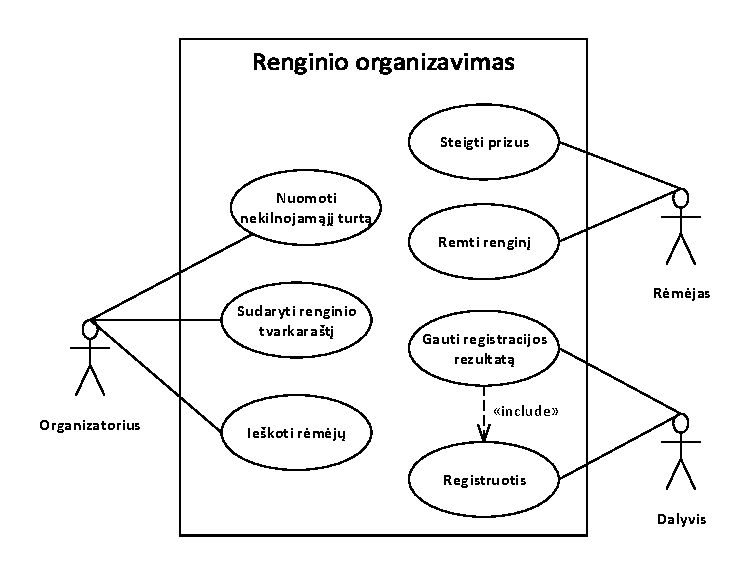
\includegraphics[width=\textwidth]{img/UzduociuDiagrama1}
          \caption{Renginio organizavimo UML užduočių diagrama}
          \label{fig:organizavimoUzduociuDiagrama}
        \end{figure}

      \subsubsubsection* {Renginio organizavimo UML užduočių diagramos aprašymas}
        \begin{enumerate}
          \item \underline{Organizatorius} \textit{nuomoja nekilnojamąjį turtą}, reikalingą sporto renginiui. Taip pat jis iš anksto \textit{sudaro renginio tvarkaraštį} bei
                \textit{ieško \underline{rėmėjų}}, kurie padėtų padengti renginio išlaidas.
          \item \underline{Rėmėjas} gali finansiškai \textit{remti renginį} bei \textit{steigti prizus} nugalėtojams.
          \item \underline{Dalyvis}, norintis dalyvauti sporto renginyje, privalo \textit{registruotis} į jį bei \textit{gauti registracijos rezultatą} iš \underline{organizatoriaus}.
        \end{enumerate}

      \subsubsubsection*{Renginio vykdymas}
        \begin{figure}[H]
          \centering
          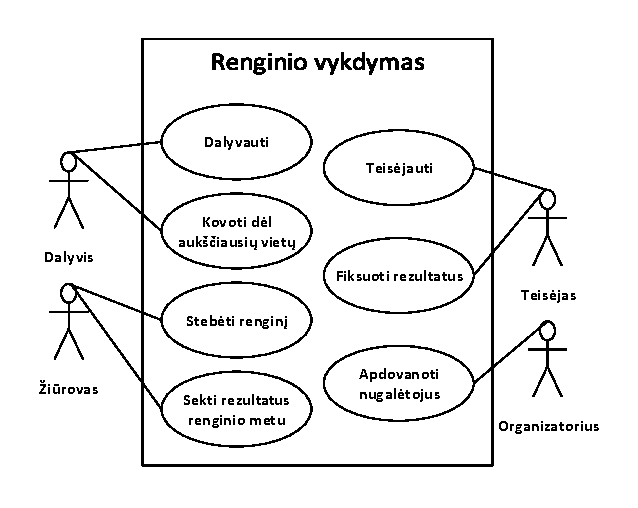
\includegraphics[width=\textwidth]{img/UzduociuDiagrama2}
          \caption{Renginio vykdymo UML užduočių diagrama}
          \label{fig:vykdymoUzduociuDiagrama}
        \end{figure}

      \subsubsubsection*{Renginio vykdymo UML užduočių diagramos aprašymas}
        \begin{enumerate}
          \item \underline{Dalyvis} \textit{dalyvauja} sporto renginyje bei \textit{kovoja dėl aukščiausių vietų}.
          \item \underline{Žiūrovas} \textit{stebi sporto renginį} bei \textit{seka \underline{dalyvių} rezultatus}.
          \item \underline{Teisėjas} \textit{teisėjauja} varžyboms bei \textit{fiksuoja \underline{dalyvių} rezultatus}.
          \item \underline{Organizatorius} į renginio vykdymą įsitraukia tik tada, kai reikia \textit{apdovanoti nugalėtojus}.
        \end{enumerate}

  \subsection{Užduočių vykdymo scenarijai} \label{vidineVersloProcesoAnalize_uzduociuVykdymoScenarijai}
    \setlist[enumerate]{label*=\arabic*.}
    %%%%%%%%%%%%%
    \subsubsection*{Registracija į sporto renginį}
      \begin{figure}[H]
        \centering
        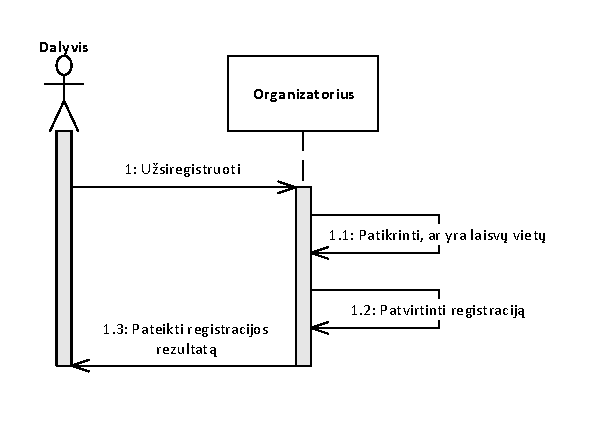
\includegraphics[width=\textwidth]{img/SekuDiagrama1}
        \caption{Registravimosi į sporto renginį UML sekų diagrama}
        \label{fig:registracijosSekuDiagrama}
      \end{figure}
      \begin{enumerate}
        \item \underline{Dalyvis} \textit{registruojasi} į sporto renginį.
          \begin{enumerate}
            \item \underline{Organizatorius} \textit{patikrina, ar yra laisvų vietų}.
            \item \underline{Organizatorius} \textit{patvirtina \underline{dalyvio} registraciją}.
            \item \underline{Organizatorius} \underline{dalyviui} \textit{pateikia registracijos rezultatą}.
          \end{enumerate}
      \end{enumerate}

    \subsubsection*{Sporto renginio organizavimas}
      \begin{figure}[H]
        \centering
        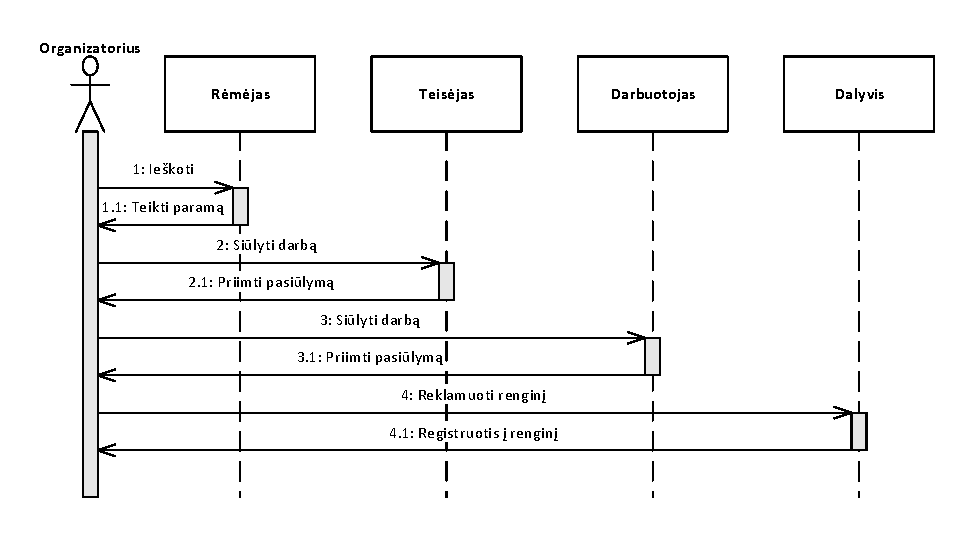
\includegraphics[width=\textwidth]{img/SekuDiagrama2}
        \caption{Sporto renginio organizavimo UML sekų diagrama}
        \label{fig:organizavimoSekuDiagrama}
      \end{figure}
      \begin{enumerate}
        \item \underline{Organizatorius} \textit{ieško \underline{rėmėjų}} sporto renginiui.
          \begin{enumerate}
            \item \underline{Rėmėjas} nusprendžia \textit{teikti paramą} \underline{organizatoriui}.
          \end{enumerate}
        \item \underline{Organizatorius} \textit{siūlo darbą} \underline{teisėjui}.
          \begin{enumerate}
            \item \underline{Teisėjas} \textit{priima darbo pasiūlymą} iš \underline{organizatoriaus}.
          \end{enumerate}
        \item \underline{Organizatorius} \textit{siūlo darbą} \underline{darbuotojui}.
          \begin{enumerate}
            \item \underline{Darbuotojas} \textit{priima darbo pasiūlymą} iš \underline{organizatoriaus}.
          \end{enumerate}
        \item \underline{Organizatorius} \textit{reklamuoja renginį}.
          \begin{enumerate}
            \item \underline{Dalyvis} pamatęs reklamą \textit{registruojasi į renginį}.
          \end{enumerate} 
      \end{enumerate}

    \subsubsection*{Sporto renginio vykdymas}
      \begin{figure}[H]
        \centering
        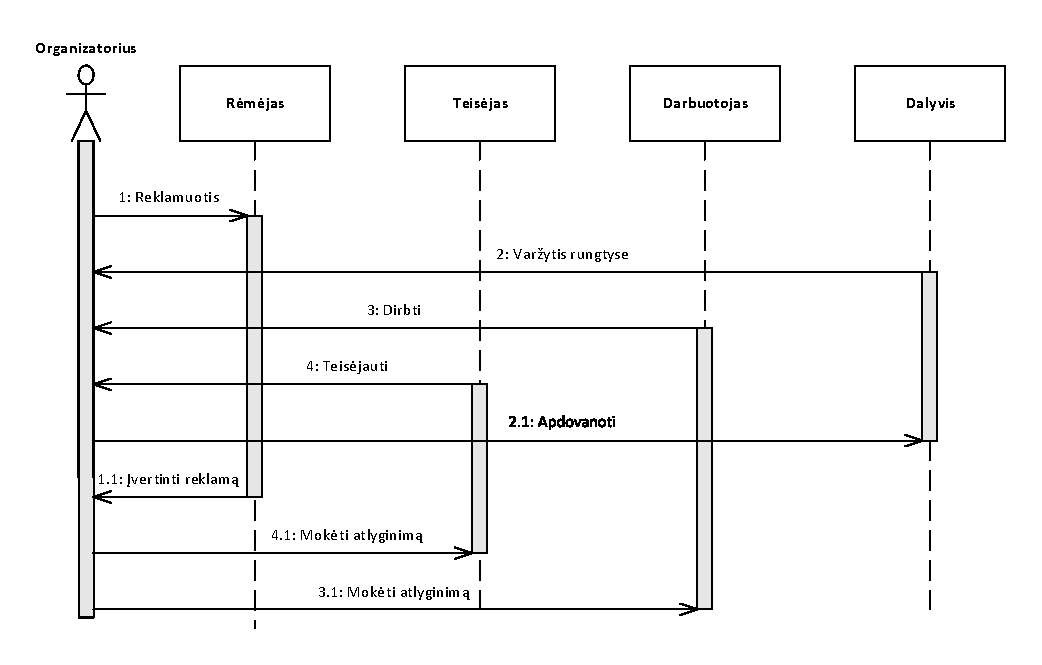
\includegraphics[width=\textwidth]{img/SekuDiagrama3}
        \caption{Sporto renginio vykdymo UML sekų diagrama}
        \label{fig:vykdymoSekuDiagrama}
      \end{figure}
      \begin{enumerate}
        \item \underline{Organizatorius} \textit{reklamuoja} \underline{rėmėjus}.
          \begin{enumerate}
            \item \underline{Rėmėjas} \underline{organizatoriui} \textit{pateikia reklamos įvertinimą}.
          \end{enumerate}
        \item \underline{Dalyvis} \textit{varžosi \underline{organizatoriaus} surengtose varžybose}.
          \begin{enumerate}
            \item \underline{Organizatorius} \textit{apdovanoja} laimėjusius \underline{dalyvius}.
          \end{enumerate}
        \item \underline{Darbuotojas} \textit{dirba} \underline{organizatoriui} - užsiima pagalbine veikla sporto renginyje.
          \begin{enumerate}
            \item \underline{Organizatorius} \textit{moka atlyginimą} \underline{darbuotojui} už atliktą darbą.
          \end{enumerate}
        \item \underline{Teisėjas} \textit{dirba} \underline{organizatoriui} - teisėjauja varžybose, matuoja ir fiksuoja rezultatus.
          \begin{enumerate}
            \item \underline{Organizatorius} \textit{moka atlyginimą} \underline{teisėjui} už atliktą darbą.
          \end{enumerate} 
      \end{enumerate}

    \subsubsection*{Dalyvavimas sporto renginyje}
      \begin{figure}[H]
        \centering
        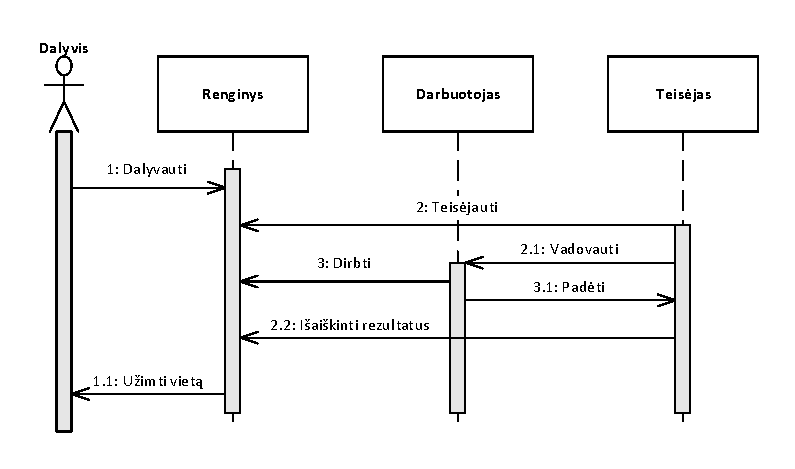
\includegraphics[width=\textwidth]{img/SekuDiagrama4}
        \caption{Dalyvavimo sporto renginyje UML sekų diagrama}
        \label{fig:dalyvavimoSekuDiagrama}
      \end{figure}
      \begin{enumerate}
        \item \underline{Dalyvis} \textit{dalyvauja} \underline{renginyje}.
          \begin{enumerate}
            \item\underline{Dalyvis} \textit{užima vietą} \underline{renginyje}.  
          \end{enumerate}
        \item \underline{Teisėjas} \textit{teisėjauja} \underline{renginiui}.
          \begin{enumerate}
            \item\underline{Teisėjas} \textit{vadovauja} \underline {darbuotojui}, paskiria jam papildomas užduotis.
            \item\underline{Teisėjas} \textit{išaiškina \underline{renginio} rezultatus} ir išskirsto dalyvius pagal juos.
            \end{enumerate}
        \item \underline{Darbuotojas} \textit{dirba} \underline{renginyje}, padeda užtikrinti sklandžią jo eigą.
          \begin{enumerate}
            \item\underline{Darbuotojas} \textit{padeda} \underline{teisėjui} prižiūrėti \underline{renginį} bei vykdo teisėjo paskirtas užduotis.
          \end{enumerate}
      \end{enumerate}

    \subsubsection*{Sporto renginio stebėjimas}
      \begin{figure}[H]
        \centering
        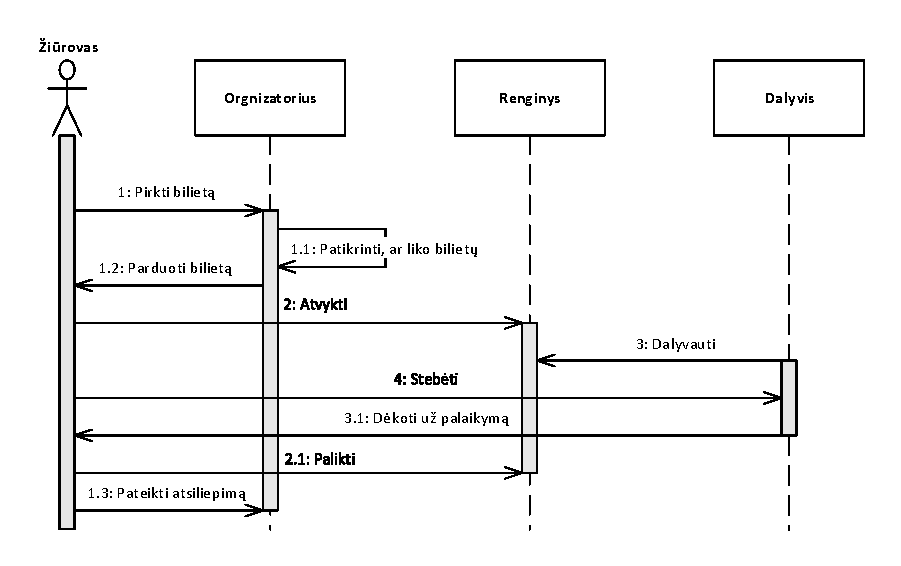
\includegraphics[width=\textwidth]{img/SekuDiagrama5}
        \caption{Sporto renginio stebėjimo UML sekų diagrama}
        \label{fig:stebejimoSekuDiagrama}
      \end{figure}
      \begin{enumerate}
        \item \underline{Žiūrovas} iš \underline{organizatoriaus}  \textit{perka bilietus} į \underline{renginį}.
          \begin{enumerate}
            \item \underline{Organizatorius} \textit{patikrina, ar liko bilietų į \underline{renginį}}.
            \item \underline{Organizatorius} \textit{parduoda bilietą} į \underline{renginį} \underline{dalyviui}.
            \item \underline{Dalyvis} \underline{organizatoriui} \textit{pateikia atsiliepimą} apie įvykusį \underline{renginį}.
          \end{enumerate}
        \item \underline{Žiūrovas} varžybų dieną \textit{atvyksta} į \underline{renginį}.
          \begin{enumerate}
            \item \underline{Žiūrovas} pasibaigus varžyboms išvyksta ir \textit{palieka} \underline{renginio} vietą.
          \end{enumerate}
        \item \underline{Dalyvis} \textit{dalyvauja} \underline{renginyje}.
          \begin{enumerate}
            \item \underline{Dalyvis} pasibaigus renginiui \textit{dėkoja} \underline{žiūrovams} už palaikymą.
          \end{enumerate}
        \item \underline{Žiūrovas} renginio metu \textit{stebi} bei palaiko \underline{dalyvius}.
      \end{enumerate}
  \subsection{Dalykinės srities dinaminė struktūra} \label{vidineVersloProcesoAnalize_dinamineStruktura}
    \subsubsection*{Dalyvio būsenos}
      \begin{figure}[H]
        \centering
        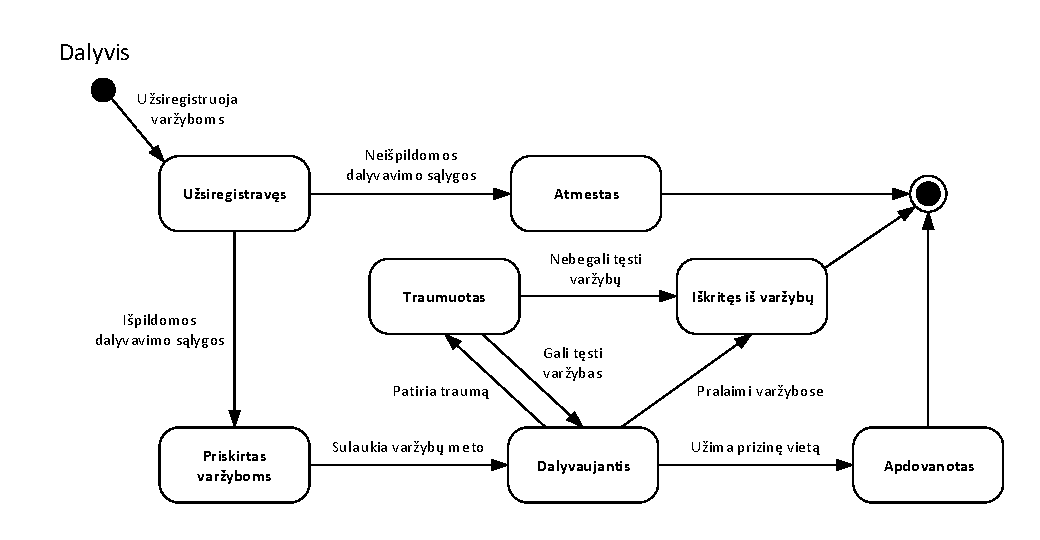
\includegraphics[width=\textwidth]{img/BusenuDiagrama1}
        \caption{Dalyvio UML būsenų diagrama}
        \label{fig:dalyvioBusenuDiagrama}
      \end{figure}
      
      \begin{itemize}
        \item \textbf{Galutinė būsena} - tai būsena, kuomet \underline{dalyvis} nedalyvauja varžybose, nes buvo atmestas, iškritęs, arba jau sudalyvavęs ir galbūt apdovanotas.
        \item \underline {Dalyvis} \textit{užsiregistruoja varžyboms}.
        \item Jei \textit{dalyvavimo sąlygos nėra išpildytos}, \underline{dalyvis} yra atmestas ir jis nebegali dalyvauti varžybose.
        \item Jei \underline{dalyvis} yra atmestas, jis patenka į \textbf{galutinę būseną}.
        \item Jei visos \textit{dalyvavimo sąlygos yra išpildytos}, \underline{dalyvis} yra priskiriamas varžyboms.
        \item Jei \underline{dalyvis} yra priskirtas varžyboms, tai jis, \textit{sulaukęs varžybų meto}, dalyvauja jos.
        \item \underline{Dalyvis}, užėmęs prizinę vietą, yra apdovanojamas.
        \item Apdovanotas \underline{dalyvis} patenka į \textbf{galutinę būseną}.
        \item \underline{Dalyvis} renginio metu gali \textit{patirti traumą}.
        \item Jei \underline{dalyvio} trauma nėra didelė, jis \textit{gali tęsti varžybas}.
        \item Stipriai traumuotas \underline{dalyvis} \textit{nebegali tęsti varžybų}, todėl jis iškrenta.
        \item \underline{Dalyvis}, kuris \textit{pralaimi varžybose}, iškrenta iš jų.
        \item Iškritęs iš varžybų \underline{dalyvis} patenka į \textbf{galutinę būseną}.
      \end{itemize}
	\subsubsection*{Žiūrovo būsenos}
	  \begin{figure}[H]
        \centering
        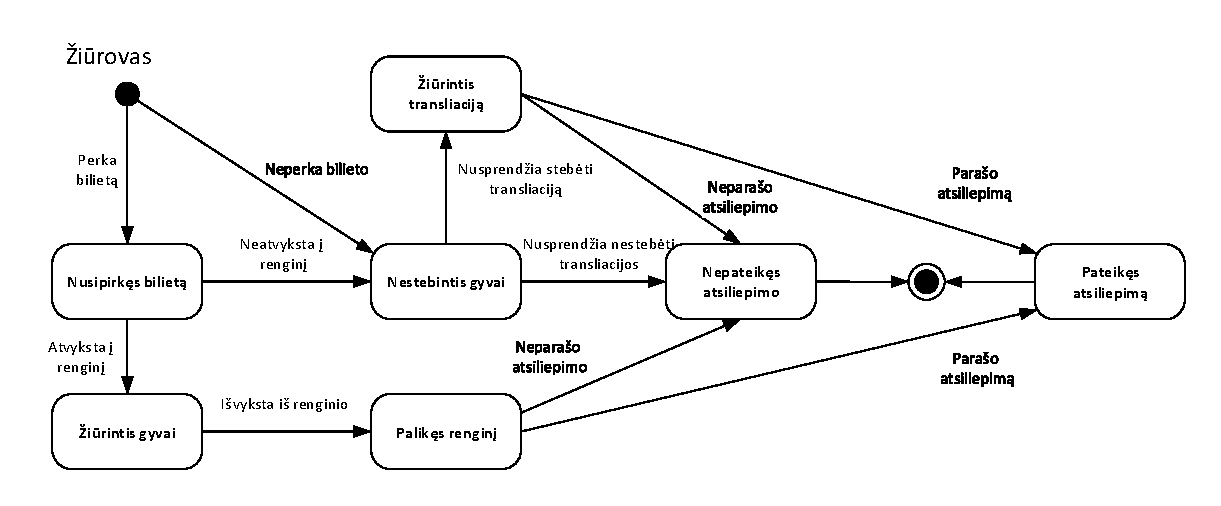
\includegraphics[width=\textwidth]{img/BusenuDiagrama2}
        \caption{Žiūrovo UML būsenų diagrama}
        \label{fig:ziurovoBusenuDiagrama}
      \end{figure}
        
      \begin{itemize}
        \item \textbf{Galutinė būsena} - tai būsena, į kurią \underline{žiūrovas} patenka pasibaigus renginiui.
        \item \underline{Žiūrovas} gali \textit{nusipirkti bilietą} į renginį.
        \item Jei \underline{žiūrovas} bilieto nenusiperka, jis negali renginio stebėti gyvai.
        \item Jei \underline{žiūrovas}, nusipirkęs bilietą, \textit{neatvyksta į renginį}, jis nebegali varžybų stebėti gyvai.
        \item \underline{Žiūrovas}, nestebėjęs renginio, \textit{atsiliepimo neparašo}.
        \item \underline{Žiūrovas}, nestebintis renginio gyvai, gali \textit{nuspręsti nestebėti transliacijos} ir dėl to tikrai nepateikia atsiliepimo.
        \item \underline{Žiūrovas}, nestebintis renginio gyvai, gali \textit{nuspręsti stebėti transliaciją}.
        \item \underline{Žiūrovas}, stebėjęs transliaciją, gali \textit{parašyti atsiliepimą} apie renginį.
        \item \underline{Žiūrovas}, stebėjęs transliaciją, gali \textit{neparašyti atsiliepimo} apie renginį.
        \item Jei \underline{žiūrovas}, nusipirkęs bilietą, \textit{atvyksta į renginį}, jis žiūri varžybas gyvai.
        \item Pažiūrėjęs renginį gyvai, \underline{žiūrovas} \textit{išvyksta iš renginio}.
        \item \underline{Žiūrovas}, palikęs renginį, gali \textit{parašyti atsiliepimą}.
        \item \underline{Žiūrovas}, palikęs renginį, gali \textit{atsiliepimo nerašyti}.
        \item Pateikęs atsiliepimą \underline{žiūrovas} patenka į \textbf{galutinę būseną}.
        \item Nepateikęs atsiliepimo \underline{žiūrovas} patenka į \textbf{galutinę būseną}.
      \end{itemize}
	\subsubsection*{Organizatoriaus būsenos}
	  \begin{figure}[H]
      \centering
      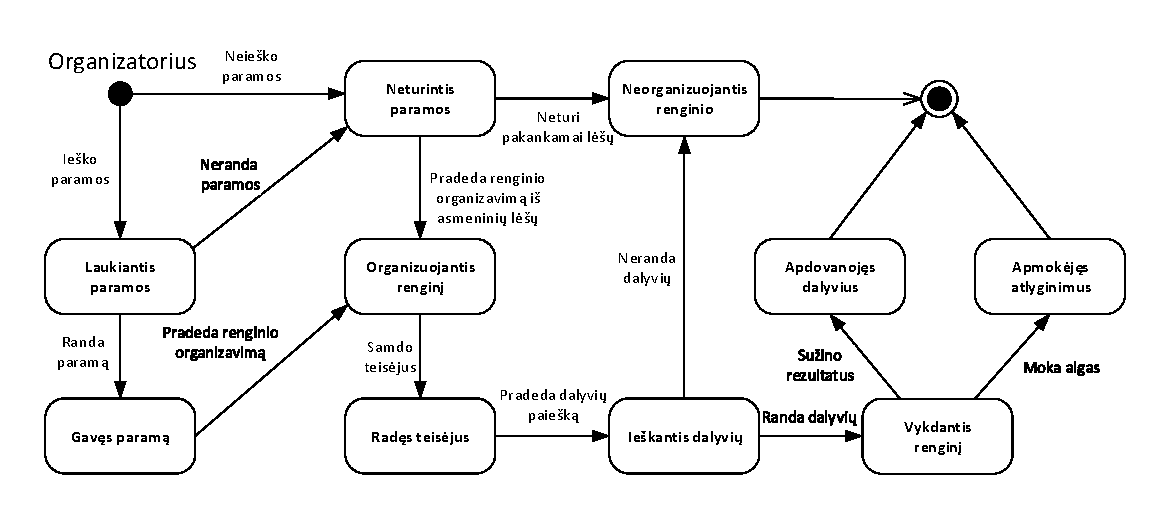
\includegraphics[width=\textwidth]{img/BusenuDiagrama3}
      \caption{Organizatoriaus UML būsenų diagrama}
      \label{fig:organizatoriausBusenuDiagrama}
    \end{figure}

    \begin{itemize}
      \item \textbf{Galutinė būsena} - tai būsena, į kurią patenka \underline{organizatorius}, apdovanojęs dalyvius bei apmokėjęs atlyginimus. Taip pat, į šią būseną patenka neorganizuojantis renginio \underline{organizatorius}.
      \item \underline{Organizatorius}, kuris \textit{neieško paramos}, jos neturi.
      \item Jei \underline{organizatorius}, neturintis paramos, \textit{neturi pakankamai lėšų} renginio organizavimui, tai jis renginio ir neorganizuoja.
      \item Neorganizuojantis renginio \underline{organizatorius} patenka į \textbf{galutinę būseną}.
      \item Neturintis paramos \underline{organizatorius} gali \textit{pradėti renginio organizavimą iš asmeninių lėšų}.
      \item \underline{Organizatorius} pradeda \textit{ieškoti paramos} ir jos laukia.
      \item \underline{Organizatorius}, kuris \textit{neranda paramos}, jos ir neturi.
      \item \underline{Organizatorius}, kuris \textit{randa paramą}, ją gauna.
      \item Gavęs paramą \underline{organizatorius} \textit{pradeda renginio organizavimą}.
      \item Organizuojantis renginį \underline{organizatorius} \textit{samdo teisėjus}.
      \item Radęs teisėjus \underline{organizatorius} \textit{pradeda dalyvių paiešką}.
      \item \underline{Organizatorius}, kuris \textit{neranda dalyvių}, renginio neorganizuoja.
      \item \underline{Organizatorius}, \textit{radęs dalyvių}, vykdo renginį.
      \item Pasibaigus renginiui \underline{organizatorius} \textit{sužino rezultatus} ir apdovanoja dalyvius.
      \item Pasibaigus renginiui \underline{organizatorius} \textit{moka algas} darbuotojams.
      \item \underline{Organizatorius}, apdovanojęs dalyvius bei apmokėjęs atlyginimus, patenka į \textbf{galutinę būseną}.
    \end{itemize}

\section{Analizės rezultatai SSGG (SWOT)} \label{analizesRezultatai}              % [TODO] patikrint reference'us, gal perdaryt jei spesim
    \begin{longtable}{@{\extracolsep{\fill}} | m{.08\hsize} | p{7cm} | p {6cm} | @{}}
      \caption{Analizės rezultatai}
      \label{table:swot}
      \endfirsthead
      \endhead
      \hline
      {} & Teigiami & Neigiami \\
      \hline
      Vidinė analizė 	& Stiprybės:
                        \begin{itemize}
                          \item Žiūrovui nėra sunku gauti bilietą - jam tereikia internetu arba vietoje nusipirkti jį iš organizatoriaus ir nuvykti į renginį (žr. \ref{fig:stebejimoSekuDiagrama} pav.)
                          \item Jeigu kyla problemų, labai aišku į ką kreiptis - viską valdo organizatorius (žr. \ref{fig:klasiuDiagrama} pav.)
                        \end{itemize}
                      & Silpnybės:
                        \begin{itemize}
                          \item Organizatorius yra labai užimtas, jam tenka daug darbo, kurį galėtų įvykdyti kitos instancijos (žr. \ref{fig:klasiuDiagrama} pav.) 
                          \item Organizuojant renginį organizatorius yra pagrindinė ir vienintelė figūra, kuri atsakinga už darbą su visomis kitomis esybėmis (žr. \ref{fig:organizavimoSekuDiagrama} pav.)
                          \item Vykdant renginį organizatorius taip pat turi daugiausiai veiklos ir yra atsakingas už visą vykdymą (žr. \ref{fig:vykdymoSekuDiagrama} pav.)
                          \item Teisėjas turi daug atsakomybės, jam tenka prižiūrėti kitus darbuotojus, kad renginys vyktų sklandžiai (žr. \ref{fig:dalyvavimoSekuDiagrama} pav.)
                          \item Dalyviui sunku užsiregistruoti į renginį, nes jam reikia susirasti organizatorių ir jam siųsti duomenis. Tai gali būti labai nepatogu, nesaugu, o kartais ir neįmanoma (žr. \ref{fig:registracijosSekuDiagrama} pav.)
                        \end{itemize}
                        \\
      \hline
      Išorinė analizė	& Galimybės:
                        \begin{itemize}
                          \item Naujas projektas gali pritraukti didelį rėmėjų palaikymą (žr. \ref{table:ieiga} lentelę).
                          \item Žiūrovai, pastebėję dalyvių gausą ir konkurenciją, susidomės žaidynėmis ir atneš pelną organizacijai žiūrėdami jas (žr. \ref{table:ieiga} ir \ref{table:reguliavimas} lenteles).
                          \item Visi Lietuvos piliečiai galėtų siūlyti naujas idėjas žaidynėms, todėl renginys gali pritraukti žmonių, nesidominčių sportu, tačiau turinčių naujų idėjų (žr. \ref{table:iseiga} lentelę).
                          \item Lietuvoje nėra vykdomos didelio masto žaidynės, į kurių sudėtį įeitų plati įvairovė sporto šakų, todėl tai būtų puiki galimybė organizacijai pradėti naują sporto tradiciją šalyje (žr. \ref{table:iseiga} lentelę).
                          \item Tam, kad būtų išvengta tiesioginio transliavimo problemų, organizacija planuoja tartis su keliais televizijos bei interneto transliuotojais (žr. \ref{isorineVersloProcesoAnalize_esamuSistemuAnalize} skyrių).
                          \item Žiūrovų poreikiams užtikrinti visos varžybos galėtų būti transliuojamos tiesiogiai. Taip pat varžybų vaizdo įrašus ir gražiausius momentus būtų galima pamatyti internete (žr. \ref{table:iseiga} lentelę).
                        \end{itemize}
                      & Grėsmės:
                        \begin{itemize}
                          \item Rėmėjų bei lėšų trūkumas gali neleisti žaidynėms iš viso įvykti (žr. \ref{table:reguliavimas} lentelę).
                          \item Nepakankamas dalyvių skaičius mažintų žiūrovų lankomumą ir dalyvių palaikymą (žr. \ref{table:ieiga} lentelę).
                          \item Mažas susidomėjimas ir populiarumo stoka gali atbaidyti rėmėjus ir stipriai sumažinti gaunamų finansų kiekį (žr. \ref{table:ieiga} lentelę).
                          \item Žiūrovų bei dalyvių atsiliepimuose paminėti žaidynių trūkumai gali būti sunkiai ištaisomi bei mažinti renginio populiarumą (žr. \ref{table:iseiga} lentelę).
                        \end{itemize}
                        \\
      \hline
    \end{longtable}
\section{Verslo proceso tobulinimo strategija} \label{versloProcesoTobulinimoStrategija}
	\subsection{Organizacijos misija} \label{versloProcesoTobulinimoStrategija_vizija}
		Organizuoti vieną iš svarbiausių sporto renginių šalies mastu, kuris apimtų kuo didesnę sportinių šakų dalį ir būtų prieinamas kuo daugiau Lietuvos piliečių.
	\subsection{Organizacijos vizija} \label{versloProcesoTobulinimoStrategija_misija}
		Populiarinti sportą Lietuvoje, į sportinę veiklą įtraukti kuo daugiau žmonių ir skatinti sveiką gyvenimo būdą.
	\subsection{Bendroji tobulinimo strategija} \label{versloProcesoTobulinimoStrategija_bendroji}
		\begin{itemize}
			\item Palengvinti organizatorių darbą ir apmažinti organizacinės veiklos kiekį.
      \item Suteikti galimybę piliečiams laisvai siūlyti naujas idėjas renginiui, kad kiekvieno balsas būtų išgirstas.
      \item Pagerinti reklamos metodiką ir informacijos platinimą, kad renginio naujienos lengviau pasiektų visuomenę ir į sportinę veiklą įsitrauktų kuo daugiau žmonių.
      \item Kontroliuoti finansų gavimą ir panaudojimą, taip užtikrinant skaidrų pinigų išskirstymą renginio tikslams.
      \item Į renginį įtraukti ir netradicines sporto šakas, siekiant jas populiarinti Lietuvoje ir pritraukti daugiau entuziastų. 
		\end{itemize}
	\subsection{Struktūrizuota tobulinimo strategija} \label{versloProcesoTobulinimoStrategija_strukturizuota}
			\begin{itemize}
				\item \textbf{Renginio populiarinimas:}
          \begin{itemize}
            \item Kvietimai dalyvauti, skelbiami socialiniuose tinkluose.
            \item Reklamos televizijoje.
            \item Naujienlaiškiai į elektroninį paštą.
            \item Garsių sportininkų atsiliepimai apie renginį.
            \item Gerinti renginio transliavimo metodus:
              \begin{itemize}
                \item Transliuoti varžybas organizacijos internetinėje svetainėje nemokamai;
                \item Laikyti visų varžybų įrašus svetainėje vėlesnei peržiūrai;
                \item Suteikti transliavimo leidimus visoms televizijos kompanijoms, rodančioms susidomėjimą renginiu.
              \end{itemize}
            \item Įsteigti prizus visiems dalyviams, o nugalėtojams - specialius, taip didinant žmonių norą dalyvauti renginyje.
          \end{itemize}
        \item \textbf{Finansų kontrolė:}
          \begin{itemize}
            \item Sudaryti konkrečius planus, kuriuose nurodoma kaip ir kur bus naudojami organizacijos finansai.
            \item Finansinius planus viešinti siekiant išlaikyti skaidrumą ir visuomenės pasitikėjimą.
            \item Riboti rėmėjų skiriamų lėšų kiekį siekiant išvengti papirkinėjimo.
          \end{itemize}
        \item \textbf{Organizacinio proceso lengvinimas:}
          \begin{itemize}
            \item Panaudoti informacinę sistemą siekiant:
              \begin{itemize}
                \item Vykdyti dalyvių registraciją;
                \item Prekiauti bilietais į renginį;
                \item Ieškoti rėmėjų;
                \item Samdyti darbuotojus.
              \end{itemize}
          \end{itemize}
        \item \textbf{Naujų idėjų siūlymas:}
          \begin{itemize}
            \item Pasitelkti informacinę sistemą, kuri kiekvienam piliečiui suteiktų galimybę:
              \begin{itemize}
                \item Prisijungti prie sistemos;
                \item Įrašyti naują pasiūlymą, kaip būtų galima gerinti renginį;
                \item Išsiųsti pasiūlymą organizatoriams;
                \item Peržiūrėti pateiktos idėjos svarstymo verdiktą - ar idėja buvo atmesta, ar priimta ir bus įgyvendinta.
              \end{itemize}
            \item Įsteigti komitetą, atsakingą už piliečių pateiktų idėjų svarstymą.
            \item Komiteto atrinktus pasiūlymus įgyvendinti per organizatorių.
            \item Piliečius, kurių pasiūlymai atrinkti įgyvendinimui, adekvačiai apdovanoti.
          \end{itemize}
        \item \textbf{Netradicinių sporto šakų įtraukimas į renginį:}
          \begin{itemize}
            \item Į renginį įtraukti ne tik įprastas sporto šakas, bet ir naujas, kurių varžybos Lietuvoje ar net pasaulyje dar nevyksta.
            \item Skirti kiek didesnį finansavimą modernių sporto šakų varžyboms, taip siekiant populiarinti šias sporto šakas visuomenėje ir sudominti jomis kuo daugiau žmonių.
            \item Pradėti naujas inovatyvių sporto šakų varžybų tradicijas.
          \end{itemize}
			\end{itemize}
\section{Sistemos naudojimo scenarijus} \label{sistemosNaudojimoScenarijus}
  \subsection{Scenarijus} \label{sistemosNaudojimoScenarijus_scenarijus}
    \subsubsection*{Renginio organizavimas}
	    \begin{figure}[H]
        \centering
        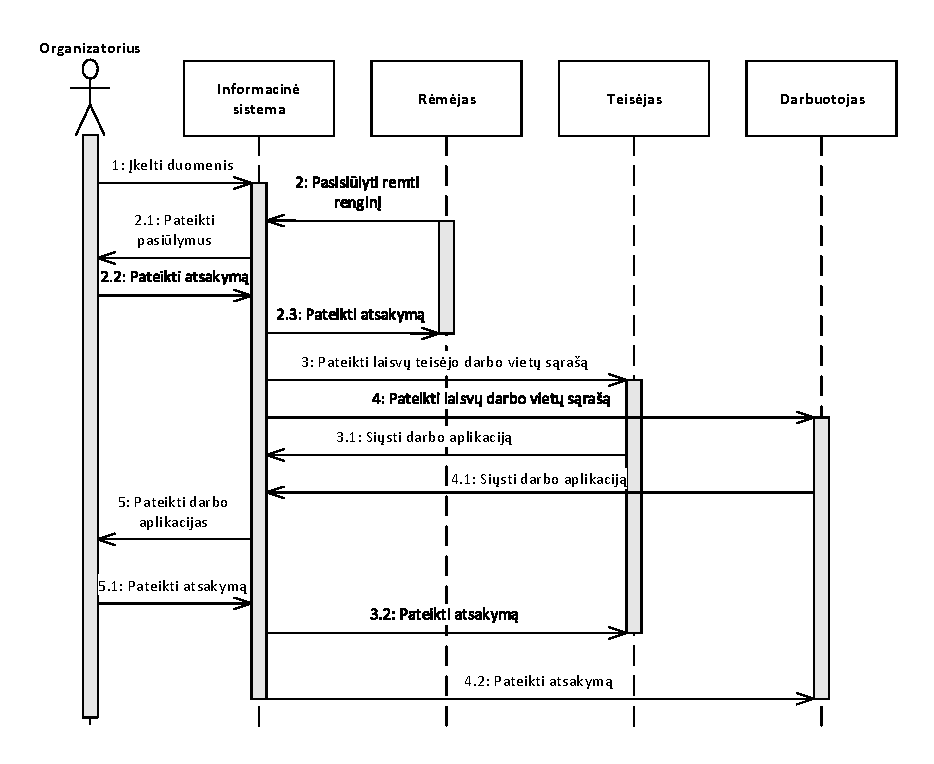
\includegraphics[width=\textwidth]{img/ScenarijausSekuDiagrama1}
        \caption{Renginio organizavimo UML sekų diagrama}
        \label{fig:scenarijusOrganizavimoSekuDiagrama}
      \end{figure}

      \begin{enumerate}
        \item \underline{Organizatorius} į \underline{informacinę sistemą} \textit{įkelia renginio duomenis} - galimas sporto šakas, tvarkaraščius, laisvų vietų skaičių, kiekvienos sporto šakos varžybų vietą ir t.t. 
        \item \underline{Rėmėjas} \underline{informacinėje sistemoje} \textit{pasisiūlo remti renginį}. 
          \begin{enumerate}
            \item \underline{Informacinėje sistemoje} esantys \underline{rėmėjų} pasiūlymai yra \textit{pateikiami} \underline{organizatoriui}.
            \item \underline{Organizatorius}, apsvarstęs pateiktą rėmėjo pasiūlymą, \textit{pateikia atsakymą}, t.y. paramos pasiūlymą priima arba atmeta, \underline{informacinėje sistemoje}.
            \item \underline{Informacinėje sistemoje} yra \textit{pateikiamas \underline{organizatoriaus} atsakymas}, kurį gali peržiūrėti \underline{rėmėjas}.
          \end{enumerate}
        \item \underline{Informacinėje sistemoje} \textit{pateikiamas laisvų teisėjo darbo vietų sąrašas}, kurį potencialus \underline{teisėjas} gali peržvelgti.
          \begin{enumerate}
            \item Potencialus \underline{teisėjas} \textit{siunčia darbo aplikaciją} į \underline{informacinę sistemą}.
            \item \underline{Teisėjas} peržiūri \underline{informacinėje sistemoje} \textit{pateiktą atsakymą}.
          \end{enumerate}
        \item \underline{Informacinėje sistemoje} \textit{pateikiamas laisvų darbo vietų sąrašas}, kurį gali peržiūrėti potencialus \underline{darbuotojas}.
          \begin{enumerate}
            \item Potencialus \underline{darbuotojas} \textit{siunčia darbo aplikaciją} į \underline{informacinę sistemą}.
            \item \underline{Darbuotojas} peržiūri \underline{informacinėje sistemoje} \textit{pateiktą atsakymą}.
          \end{enumerate}
        \item \underline{Organizatorius} peržiūri \underline{informacinėje sistemoje} \textit{pateiktas darbo aplikacijas}.
          \begin{enumerate}
            \item \underline{Organizatorius}, apsvarstęs darbo aplikacijas, išsirenka geriausius kandidatus ir jų aplikacijas patvirtina, o kitas atmeta. Tada \textit{pateikia atsakymą}  \underline{informacinėje sistemoje}.
          \end{enumerate}
      \end{enumerate}

    \subsubsection*{Dalyvavimas renginyje}
	    \begin{figure}[H]
        \centering
        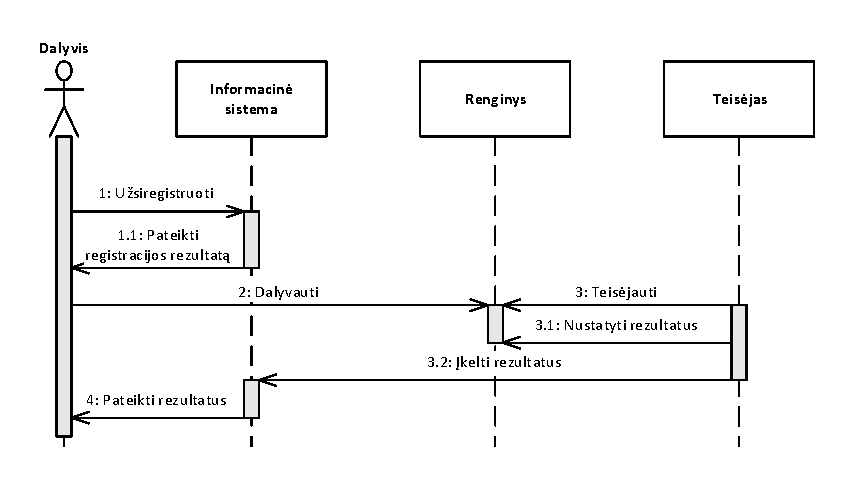
\includegraphics[width=\textwidth]{img/ScenarijausSekuDiagrama2}
        \caption{Dalyvavimo renginyje UML sekų diagrama}
        \label{fig:scenarijusDalyvavimoSekuDiagrama}
      \end{figure}
      
      \begin{enumerate}
        \item  \underline{Dalyvis}, pasirinkęs rungtį, kurioje nori dalyvauti, \textit{užsiregiztruoja} \underline{informacinėje sistemoje}.
          \begin{enumerate}
            \item \underline{Dalyvis} peržiūri \underline{informacinėje sistemoje}  \textit{pateiktą registracijos rezultatą}. Jis gali būti tiek teigiamas, kai
                  registracija buvo sėkminga, tiek neigiamas, jei įvyko kažkokia klaida (pavyzdžiui, nebeliko laisvų vietų).
          \end{enumerate}
        \item \underline{Dalyvis} \textit{dalyvauja} \underline{renginyje} ir varžosi dėl prizinių vietų.
        \item \underline{Teisėjas} \textit{teisėjauja} \underline{renginyje}. Jam padeda kiti darbuotojai, kurie rūpinasi, kad \underline{renginys} vyktų sklandžiai. 
          \begin{enumerate}
            \item \underline{Teisėjas} \underline{renginio} metu fiksuoja bei  \textit{nustato rezultatus}.
            \item  \underline{Teisėjo} fiksuoti  \textit{rezultatai įkeliami} į \underline{informacinę sistemą}.
          \end{enumerate}
        \item \underline{Dalyvis} gali peržiūrėti \underline{informacinėje sistemoje}  \textit{pateiktus rezultatus}. 
      \end{enumerate}
      
    \subsubsection*{Naujo pasiūlymo teikimas}
	    \begin{figure}[H]
        \centering
        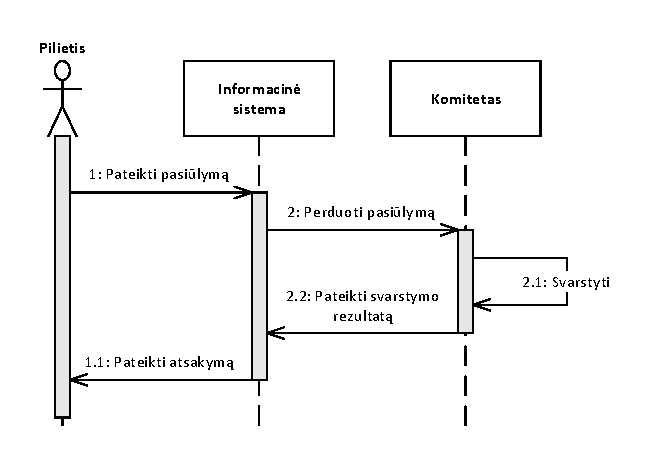
\includegraphics[width=\textwidth]{img/ScenarijausSekuDiagrama3}
        \caption{Naujo pasiūlymo teikimo UML sekų diagrama}
        \label{fig:scenarijusPasiulymoSekuDiagrama}
      \end{figure}
      
      \begin{enumerate}
        \item \underline{Pilietis}, turintis naują idėją varžyboms, \textit{pateikia pasiūlymą} \underline{informacinėje sistemoje}.
          \begin{enumerate}
            \item \underline{Informacinė sistema} \underline{piliečiui} \textit{pateikia atsakymą} apie jo pateiktą pasiūlymą.
          \end{enumerate}
        \item \underline{Informacinės sistemos} dėka, naujas pasiūlymas \textit{perduodamas} \underline{komitetui}.
          \begin{enumerate}
            \item \underline{Komitetas} \textit{svarsto} naują pasiūlymą, t.y. sprendžia, ar pasiūlymą apsimoka įgyvendinti, ar jis atsipirks, patiks žiūrovams bei dalyviams ir pan.
            \item \underline{Komitetas} \textit{pateikia svarstymo rezultatą} \underline{informacinėje sistemoje}.
          \end{enumerate}
      \end{enumerate}
      
  \subsection{Sistemos teikiama nauda} \label{sistemosNaudojimoScenarijus_nauda}
    \subsubsection*{Organizacijos viduje}
	    \begin{figure}[H]
        \centering
        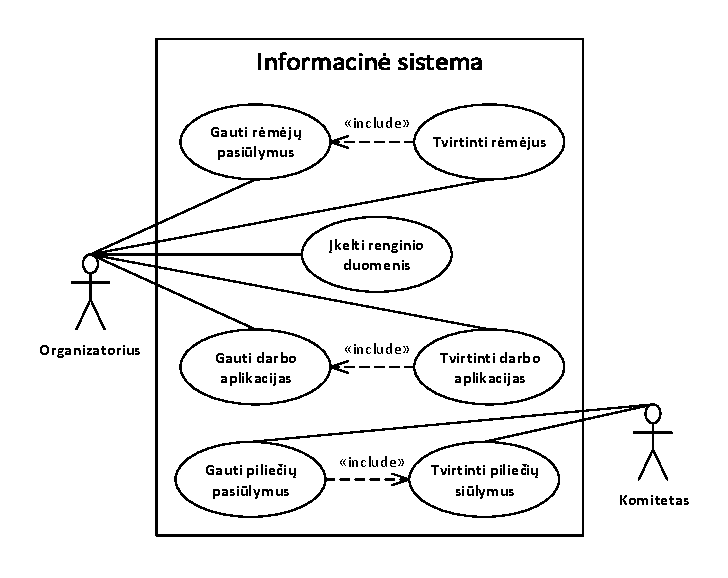
\includegraphics[width=\textwidth]{img/ScenarijausUzduociuDiagrama1}
        \caption{Sistemos teikiamos naudos organizacijos viduje UML užduočių diagrama}
        \label{fig:scenarijusVidausUzduociuDiagrama}
      \end{figure}

      \begin{enumerate}
        \item \underline{Organizatorius}, pasitelkęs informacinę sistemą:
          \begin{itemize}
            \item \textit{Gauna rėmėjų pasiūlymus}. Gavęs juos, \underline{organizatorius} apsvarsto pateiktus pasiūlymus bei  \textit{tvirtina rėmėjus}.
            \item \textit{Įkelia renginio duomenis} į informacinę sistemą.
            \item \textit{Gauna darbo aplikacijas}. Gavęs jas, \underline{organizatorius} apsvarsto bei  \textit{tvirtina darbo aplikacijas} - pateikia teigiamą ar neigiamą atsakymą, priklausomai nuo asmens aplikacijos.
          \end{itemize}
        \item \underline{Komitetas}, pasitelkęs informacinę sistemą:
          \begin{itemize}
            \item \textit{Gauna piliečių pasiūlymus} su naujomis idėjomis varžybų organizavimui. Apsvarstęs juos, \underline{komitetas} \textit{tvirtina piliečių pasiūlymus}.
          \end{itemize}
      \end{enumerate}

    \subsubsection*{Už organizacijos ribų}
	    \begin{figure}[H]
        \centering
        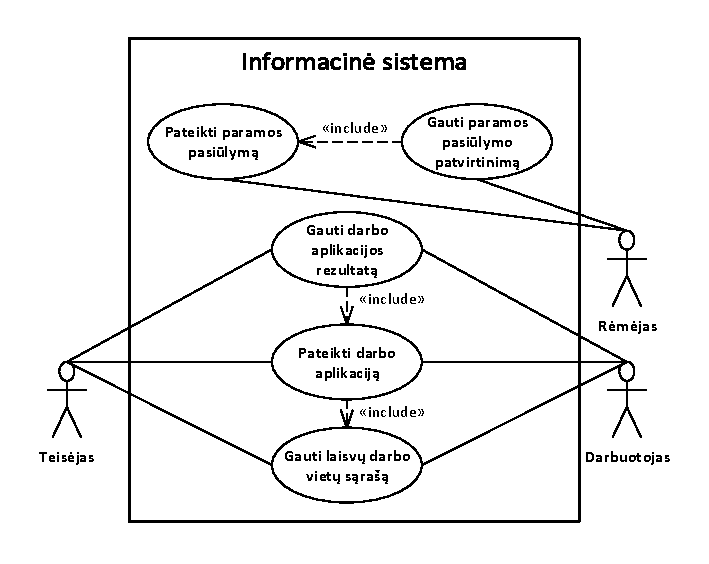
\includegraphics[width=\textwidth]{img/ScenarijausUzduociuDiagrama2}
        \caption{Sistemos išoriniams vykdytojams teikiamos naudos UML užduočių diagrama}
        \label{fig:scenarijusIsoresVykdytojuUzduociuDiagrama}
      \end{figure}

      \begin{enumerate}
        \item \underline{Rėmėjas}, pasitelkęs informacinę sistemą:
          \begin{itemize}
            \item \textit{Pateikia paramos pasiūlymą}. Tuomet \underline{rėmėjas} laukia, kol organizatoriai apsvartys jo išsakytas
                  idėjas. Organizatoriams nusprendus priimti paramą, \underline{rėmėjas} \textit{gauna pasiūlymo patvirtinimą}.
          \end{itemize}
        \item \underline{Teisėjas}, pasitelkęs informacinę sistemą:
          \begin{itemize}
            \item \textit{Gauna laisvų} \underline{teisėjo} \textit{darbo vietų sąrašą}. Gavęs sąrašą, \underline{teisėjas}
                  \textit{pateikia darbo aplikaciją} informacinėje sistemoje. Organizatoriui apsvarsčius ir nusprendus dėl
                  įdarbinimo, \underline{teisėjas} \textit{gauna darbo aplikacijos rezultatą}.
          \end{itemize}
        \item \underline{Darbuotojas}, pasitelkęs informacinę sistemą:
          \begin{itemize}
            \item \textit{Gauna laisvų} įvairaus \textit{pagalbinio darbo vietų sąrašą}. Gavęs sąrašą, pagalbinis \underline{darbuotojas}
                  \textit{pateikia darbo aplikaciją} informacinėje sistemoje. Organizatoriui apsvarsčius aplikaciją, \underline{darbuotojas}
                  \textit{gauna darbo aplikacijos rezultatą}.
          \end{itemize}
      \end{enumerate}
      
	    \begin{figure}[H]
        \centering
        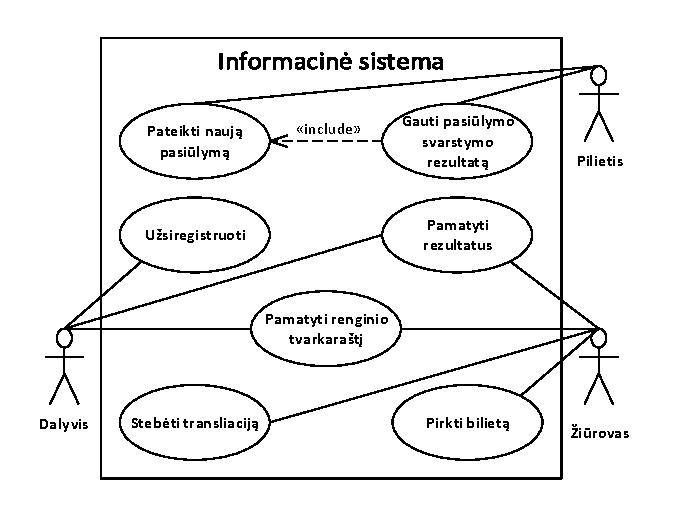
\includegraphics[width=\textwidth]{img/ScenarijausUzduociuDiagrama3}
        \caption{Sistemos išoriniams naudotojams teikiamos naudos UML užduočių diagrama}
        \label{fig:scenarijusIsoresNaudotojuUzduociuDiagrama}
      \end{figure}

      \begin{enumerate}
        \item \underline{Pilietis}, pasitelkęs informacinę sistemą:
          \begin{itemize}
            \item \textit{Pateikia naują pasiūlymą}. Komitetui apsvarsčius \underline{piliečio} pateiktą pasiūlymą, \textit{gauna pasiūlymo svarstymo rezultatą}.
          \end{itemize}
        \item \underline{Dalyvis}, pasitelkęs informacinę sistemą:
          \begin{itemize}
            \item \textit{Užsiregistruoja} į norimas varžybas.
            \item Pasibaigus varžyboms, sistemoje \textit{pamato rezultatus}.
          \end{itemize}
        \item \underline{Žiūrovas}, pasitelkęs informacinę sistemą gali:
          \begin{itemize}
            \item \textit{Pamatyti} būsimų \textit{varžybų renginio tvarkaraštį}.
            \item Pasibaigus varžyboms sistemoje \textit{pamatyti dalyvių rezultatus}.
            \item \textit{Stebėti} tiesioginę ar įrašytą varžybų \textit{transliaciją}.
            \item \textit{Pirkti bilietą} į renginį.
          \end{itemize}
      \end{enumerate}

  \subsection{Esama būklė} \label{sistemosNaudojimoScenarijus_esamaBukle}
    \subsubsection*{Esama įmonės infrastruktūra} \label{sistemosNaudojimoScenarijus_esamaBukle_esamaInfrastruktura}
      \begin{itemize}
        \item 4 darbuotojai
        \item 4 kompiuteriai
      \end{itemize}
    \subsubsection*{Priemonės, kurių gali prireikti} \label{sistemosNaudojimoScenarijus_esamaBukle_priemonesKuriuGaliPrireikti}
      \begin{itemize}
        \item Kompiuteris
        \item Interneto prieiga
        \item Telefonas
        \item Planšetinis kompiuteris
        \item Mobilusis ryšys
      \end{itemize}	
    \subsection{Priemonės scenarijui įgyvendinti} \label{sistemosNaudojimoScenarijus_esamaBukle_priemonesScenarijuiIgyvendinti}
      \begin{itemize}
        \item Reikiamos licencijos:
          \begin{itemize}
            \item XCode
            \item Windows Microsoft OS
            \item Android Studio
            \item Visual Studio Professional
          \end{itemize}
        \item Įranga kūrimui ir testavimui:
          \begin{itemize}
            \item Kompiuteris su MacOS
            \item Kompiuteris su Windows OS
            \item Telefonas ir planšetinis kompiuteris su:
              \begin{itemize}
                \item iOS
                \item Windows OS
                \item Android OS
              \end{itemize}
          \end{itemize}
        \item Serveris duomenų saugojimui ir svetainės hostingui  % [TODO] ar "hostingas" tikrai vartotinas?
        \item Domenas interneto svetainės talpinimui
        \item ,,Pluralsight'' prenumerata personalo apmokymui
      \end{itemize}

\section{Įgyvendinamumo ir naudos analizė} \label{igyvendinamumoIrNaudosAnalize}
  \renewcommand{\tabularxcolumn}[1]{m{#1}}
  \subsection{Operacinis įgyvendinamumas} \label{igyvendinamumoIrNaudosAnalize_operacinis}
	\begin{table}[H]
      \caption{Operacinio įgyvendinamumo lentelė}
      \label{table:operacinisIgyvendinamumas}
      \begin{tabularx}{.9\textwidth} [t]{ | X | X |}
        \hline
			\textbf{Sistemos diegimo inovaciniai slenksčiai} & \textbf{Priemonės, kaip tokių trukdžių išvengti, ar sušvelninti jų įtaką} \\
		\hline
			Sistemos sukūrimas. Pasamdyti darbuotojai gali neišpildyti visų norimų reikalavimų. & Tam, kad sistema būtų sukurta tiksliai tokia, kokios reikalauja organizacija, darbuotojams bus iškelti aiškūs nurodymai. \\
        \hline
			Sklandaus sistemos veikimo užtikrinimas. Tiek dėl pačios sistemos, tiek dėl darbuotojų klaidų sistema gali pateikti netikslią informaciją. & Tam, kad būtų sumažinti sistemos netikslumai, bus samdomi darbuotojai, kurie nuolat testuos ir sieks kuo patogesnio bei tikslesnio veikimo. \\
		\hline
			Sistemoje gali likti senų, nereikalingų duomenų, galinčių sudaryti sunkumų tiek organizatoriams, tiek potencialiems dalyviams bei žiūrovams. & Sistemoje bus įdiegta programa, kuri automatiškai po tam tikro laiko panaikins registraciją į jau pasibaigusius renginius ir kitus nebereikalingus duomenis. \\
		\hline
			Į silpną sistemą gali įsilaužti nepageidaujami asmenys. & Tam, kad į sistemą nebūtų įsilaužta ir ji nebūtų pažeista, bus samdomi darbuotojai, užtikrinantys sistemos saugumą. \\
		\hline
      \end{tabularx}
    \end{table}
  \subsection{Techninis įgyvendinamumas} \label{igyvendinamumoIrNaudosAnalize_techninis}
	\begin{table}[H]
      \caption{Techninio įgyvendinamumo lentelė}
      \label{table:techninisIgyvendinamumas}
      \begin{tabularx} {.9\textwidth}{ | X | X |}
        \hline
			\textbf{Problemos} & \textbf{Įgyvendinimo metodai} \\
		\hline
			Esamam personalui trūksta serverių priežiūros, duomenų bazių valdymo, internetinių svetainių bei mobiliųjų aplikacijų kūrimo ir panašių įgūdžių. & Personalo apmokymas, internetinių video pamokų portalų paslaugų prenumeratų įsigijimas, individualus darbuotojų mokymasis, ekspertų pagalba. \\
		\hline
			Serveriui, internetinei renginio svetainei ir mobiliajai aplikacijai reikia nuolatinės priežiūros, kad duomenys visada būtų atnaujinti, o serveris veiktų efektyviai ir vartotojui būtų malonus naudoti. & Specialistų samdymas serverių techninei priežiūrai, gera backend sistema lengvai informacinės sistemos priežiūrai ir duomenų įvedimui, išėmimui bei keitimui. \\
		\hline
			Dalyviai ir piliečiai, norintys teikti pasiūlymus organizatoriams, turi užsiregistruoti informacinėje sistemoje ir pateikti savo asmeninius duomenis. Jei nebus užtikrintas informacinės sistemos saugumas, privatūs duomenis gali būti nutekinti. & Samdyti duomenų saugumo specialistus, apmokyti darbuotojus, kad būtų laikomasi gerų programavimo praktikų, užtikrinančių duomenų saugumą kuriamoje sistemoje. \\
		\hline
			Perkant bilietus per informacinę sistemą piniginės transakcijos gali būti perimtos trečių šalių asmenų ir vartotojo pinigai gali būti nesaugiai perduodami organizacijai. & Bendradarbiavimas su bankais, piniginių transakcijų vykdymas per jų sistemas, taip užtikrinant vartotojų pinigų saugumą. \\
		\hline
			Tiesioginės renginių transliacijos internetu gali būti lėtos, jei vienu metu žiūrės daug žmonių ar kils techninių trukdžių, kas atbaidytų žiūrovus ir mažintų renginio populiarumą. & Užtikrinamas geras ir patikimas interneto ryšys renginio vietoje, kad transliacijų medžiaga būtų greitai siunčiama. Taip pat pasirūpinama kokybiška renginio akimirkų fiksavimo įranga. \\
		\hline
			Laikui bėgant serveriuose neišvengiamai kaupsis vis daugiau informacijos: vartotojų duomenų, varžybų vaizdo įrašų ir pan. Paprastas komunikavimas su serveriu taps nepakankamai efektyvus ir užtruks per daug laiko. & Pasirūpinti efektyvių algoritmų analize ir implementavimu, kad informacinė sistema galėtų efektyviai dirbti su milžinišku kiekiu duomenų ir vartotojas nepajustų jokių šalutinių efektų. \\
		\hline
      \end{tabularx}
    \end{table}
  \subsection{Ekonominis įgyvendinamumas} \label{igyvendinamumoIrNaudosAnalize_ekonominis}
	\subsubsection*{Išlaidos}
		\begin{table}[H]
			\caption{Ekonominio įgyvendinamumo išlaidų lentelė}
			\label{table:ekonominisIgyvendinamumas_islaidos}
			\begin{tabularx} {.9\textwidth}{ | m{2cm} | m{7cm} | X |}
				\hline
					\textbf{Išlaidų etapai} & \textbf{Įgyvendinimo metodai} & \textbf{Išlaidos per sezoną} \\
				\hline 
					Arenų nuoma & Kontaktuojama su arenos savininkais. Vykdomos derybos dėl kainos ir kokybės. Išsirenkama tinkama žaidynėms data. &$ 1\,000\,000\ € $\\
				\hline
					Licencijų pirkimas & Internete ieškoma licencijų, kurios reikalingos būtinam programinės įrangos naudojimui. & $3\,000\ € $\\
				\hline
					Techninė įranga & Informacinės sistemos kūrimui (internetinė svetainė ir telefoninė aplikacija) reikalingi kompiuteriai (su Windows OS, MacOS) ir telefonai (Android, Windows Phone, iPhone). &
					Kompiuteriai: \newline
					$2 \cdot 2\,000 = 4\,000\ €$ \newline
					Telefonai: \newline
					$3 \cdot 400 = 1\,200\ €$ \\
				\hline
					Inventoriaus pirkimas bei nuoma & Varžybų vykdymui reikalinga daugybė sportinio inventoriaus, kurio dalį turės pačios arenos ir stadionai. Trūkstamus teks įsigyti ar išsinuomoti. & $100\,000\ €$ \\
				\hline
					Algų mokėjimas & Reikės mokėti atlyginimus visiems prisidėjusiems prie renginio organizavimo: Informacinės sistemos kūrėjai ir testuotojai, teisėjai, teisėjų padėjėjai, varžybų sekretoriai, pasiūlymų komiteto darbuotojai. &
					Sistemos kūrėjai: \newline
					$4 \cdot 2\,500 = 10\,000\ €$ \newline
					Testuotojai:\newline
					$2 \cdot  1\,500 = 3\,000\ €$\newline
					Darbuotojai renginiuose:\newline
					$200 \cdot  200 = 40\,000\ €$\newline
					Komiteto darbuotojai:\newline
					$4 \cdot  500 = 2\,000\ €$\newline
					Sekretoriai:\newline
					$50 \cdot  300 = 15\,000\ € $\\
				\hline
					Serverio išlaikymas & Turimus ir gaunamus duomenis reikės laikyti serveryje, kurio išlaikymas, elektra ir priežiūra taip pat kainuoja. & $500\ €$ \\
				\hline
					Domeno išpirka & Internetinei svetainei palaikyti reikalingas nupirktas domenas. & $100\ €$ \\
				\hline
					\multicolumn{2}{c|}{} & Iš viso: $1\,178\,800\ €$ \\
				\cline{3-3}
			\end{tabularx}
		\end{table}
	\subsubsection*{Pajamos}
		\begin{table}[H]
			\caption{Ekonominio įgyvendinamumo pajamų lentelė}
			\label{table:ekonominisIgyvendinamumas_pajamos}
			\begin{tabularx} {.9\textwidth}{ | X | X |}
				\hline
					\textbf{Pajamų šaltinis} & \textbf{Numatoma suma per sezoną} \\
				\hline
					Rėmėjų skiriamos lėšos renginio organizavimui & $3 \cdot 50\,000 = 150\,000\ €$ \\
				\hline
					Iš žmonių nupirktų bilietų gaunamos pajamos & $100\,000 \cdot 5 = 500\,000\ €$ \\
				\hline
					Lėšos gautos iš savivaldybių & $500\,000\ €$ \\
				\hline
					Televizijos kontraktų pasirašymas dėl tiesioginės renginio transliacijos & $3 \cdot 5\,000 = 15\,000\ €$ \\
				\hline
					\multicolumn{1}{c|}{} &  Iš viso: $1\,165\,000\ €$ \\
				\cline{2-2}
			\end{tabularx}
		\end{table}
		Pirmieji metai pagal planą yra truputį nuostolingi. Tačiau taip yra tik dėl to, kad reikia supirkti visą inventorių, o ir rėmėjai nežiūrės labai rimtai į tokį renginį, kuris vyksta pirmą kartą. Augant populiarumui, padidės ir žmonių susidomėjimas. Invertorius liks dar bent keletui metų, todėl išlaidos sumažės gana ženkliai. Taigi, antras sezonas preliminariais duomenis atneš pelno.
  \subsection{Juridinis įgyvendinamumas} \label{igyvendinamumoIrNaudosAnalize_juridinis}
	Bus perkamos licencijos darbui su elektroninėmis projekto dalimis, bei bus gauti leidimai iš sporto federacijų rengti atitinkamos sporto šakos turnyrą. Lėšos gautos iš rėmėjų, bilietų ir savivaldybių bus deklaruojamos ir visi mokesčiai skraidriai apmokami. Bus užtikrinta, kad komitetas pasiūlymus svarstytų skaidriai ir neturėtų jokių savų interesų. Sporto transliacijos bus vykdomos, tik su tomis televizijos įmonėmis, kurios sutiks pasirašyti sutartį. O visi sporto renginiai ir dalyvavimas juose yra savanoriški, todėl tam jokie teisės aktai neprieštarauja. Visi dalyviai turės pasirašyti dalyvavimo sutartį, kurioje jie sutinka su organizatorių teikiamomis sąlygomis ir neturės pretenzijų traumos ar pasikeitusių turnyro taisyklių atveju. Organizatorius užtikrina dalyvio asmeninių duomenų saugumą.
\sectionnonum{Literatūros sąrašas}
  \begin{itemize}
    \item Doc. dr. K. Petrausko Programų Sistemų Inžinerijos kurso konspektai
    \item A. Abran, J. W. Moore, P.Bourque, R. Dupuis, L. L. Tripp - ,,Guide to the Software Engineering Body of Knowledge''
    \item SWOT analizės dokumentacija \url{http://ctb.ku.edu/en/table-of-contents/assessment/assessing-community-needs-and-resources/swot-analysis/main}
    \item UML dokumentacija \url{https://www.tutorialspoint.com/uml/uml_2_overview.htm}
    \item Oficialus olimpinių žaidynių tinklalapis \url{https://www.olympic.org/}
  \end{itemize}
\end{document}
